% Options for packages loaded elsewhere
\PassOptionsToPackage{unicode}{hyperref}
\PassOptionsToPackage{hyphens}{url}
%
\documentclass[
]{article}
\usepackage{lmodern}
\usepackage{amsmath}
\usepackage{ifxetex,ifluatex}
\ifnum 0\ifxetex 1\fi\ifluatex 1\fi=0 % if pdftex
  \usepackage[T1]{fontenc}
  \usepackage[utf8]{inputenc}
  \usepackage{textcomp} % provide euro and other symbols
  \usepackage{amssymb}
\else % if luatex or xetex
  \usepackage{unicode-math}
  \defaultfontfeatures{Scale=MatchLowercase}
  \defaultfontfeatures[\rmfamily]{Ligatures=TeX,Scale=1}
\fi
% Use upquote if available, for straight quotes in verbatim environments
\IfFileExists{upquote.sty}{\usepackage{upquote}}{}
\IfFileExists{microtype.sty}{% use microtype if available
  \usepackage[]{microtype}
  \UseMicrotypeSet[protrusion]{basicmath} % disable protrusion for tt fonts
}{}
\makeatletter
\@ifundefined{KOMAClassName}{% if non-KOMA class
  \IfFileExists{parskip.sty}{%
    \usepackage{parskip}
  }{% else
    \setlength{\parindent}{0pt}
    \setlength{\parskip}{6pt plus 2pt minus 1pt}}
}{% if KOMA class
  \KOMAoptions{parskip=half}}
\makeatother
\usepackage{xcolor}
\IfFileExists{xurl.sty}{\usepackage{xurl}}{} % add URL line breaks if available
\IfFileExists{bookmark.sty}{\usepackage{bookmark}}{\usepackage{hyperref}}
\hypersetup{
  pdftitle={Análisis Estadístico Básico con R},
  hidelinks,
  pdfcreator={LaTeX via pandoc}}
\urlstyle{same} % disable monospaced font for URLs
\usepackage[margin=1in]{geometry}
\usepackage{color}
\usepackage{fancyvrb}
\newcommand{\VerbBar}{|}
\newcommand{\VERB}{\Verb[commandchars=\\\{\}]}
\DefineVerbatimEnvironment{Highlighting}{Verbatim}{commandchars=\\\{\}}
% Add ',fontsize=\small' for more characters per line
\newenvironment{Shaded}{}{}
\newcommand{\AlertTok}[1]{\textcolor[rgb]{1.00,0.00,0.00}{\textbf{#1}}}
\newcommand{\AnnotationTok}[1]{\textcolor[rgb]{0.38,0.63,0.69}{\textbf{\textit{#1}}}}
\newcommand{\AttributeTok}[1]{\textcolor[rgb]{0.49,0.56,0.16}{#1}}
\newcommand{\BaseNTok}[1]{\textcolor[rgb]{0.25,0.63,0.44}{#1}}
\newcommand{\BuiltInTok}[1]{#1}
\newcommand{\CharTok}[1]{\textcolor[rgb]{0.25,0.44,0.63}{#1}}
\newcommand{\CommentTok}[1]{\textcolor[rgb]{0.38,0.63,0.69}{\textit{#1}}}
\newcommand{\CommentVarTok}[1]{\textcolor[rgb]{0.38,0.63,0.69}{\textbf{\textit{#1}}}}
\newcommand{\ConstantTok}[1]{\textcolor[rgb]{0.53,0.00,0.00}{#1}}
\newcommand{\ControlFlowTok}[1]{\textcolor[rgb]{0.00,0.44,0.13}{\textbf{#1}}}
\newcommand{\DataTypeTok}[1]{\textcolor[rgb]{0.56,0.13,0.00}{#1}}
\newcommand{\DecValTok}[1]{\textcolor[rgb]{0.25,0.63,0.44}{#1}}
\newcommand{\DocumentationTok}[1]{\textcolor[rgb]{0.73,0.13,0.13}{\textit{#1}}}
\newcommand{\ErrorTok}[1]{\textcolor[rgb]{1.00,0.00,0.00}{\textbf{#1}}}
\newcommand{\ExtensionTok}[1]{#1}
\newcommand{\FloatTok}[1]{\textcolor[rgb]{0.25,0.63,0.44}{#1}}
\newcommand{\FunctionTok}[1]{\textcolor[rgb]{0.02,0.16,0.49}{#1}}
\newcommand{\ImportTok}[1]{#1}
\newcommand{\InformationTok}[1]{\textcolor[rgb]{0.38,0.63,0.69}{\textbf{\textit{#1}}}}
\newcommand{\KeywordTok}[1]{\textcolor[rgb]{0.00,0.44,0.13}{\textbf{#1}}}
\newcommand{\NormalTok}[1]{#1}
\newcommand{\OperatorTok}[1]{\textcolor[rgb]{0.40,0.40,0.40}{#1}}
\newcommand{\OtherTok}[1]{\textcolor[rgb]{0.00,0.44,0.13}{#1}}
\newcommand{\PreprocessorTok}[1]{\textcolor[rgb]{0.74,0.48,0.00}{#1}}
\newcommand{\RegionMarkerTok}[1]{#1}
\newcommand{\SpecialCharTok}[1]{\textcolor[rgb]{0.25,0.44,0.63}{#1}}
\newcommand{\SpecialStringTok}[1]{\textcolor[rgb]{0.73,0.40,0.53}{#1}}
\newcommand{\StringTok}[1]{\textcolor[rgb]{0.25,0.44,0.63}{#1}}
\newcommand{\VariableTok}[1]{\textcolor[rgb]{0.10,0.09,0.49}{#1}}
\newcommand{\VerbatimStringTok}[1]{\textcolor[rgb]{0.25,0.44,0.63}{#1}}
\newcommand{\WarningTok}[1]{\textcolor[rgb]{0.38,0.63,0.69}{\textbf{\textit{#1}}}}
\usepackage{graphicx}
\makeatletter
\def\maxwidth{\ifdim\Gin@nat@width>\linewidth\linewidth\else\Gin@nat@width\fi}
\def\maxheight{\ifdim\Gin@nat@height>\textheight\textheight\else\Gin@nat@height\fi}
\makeatother
% Scale images if necessary, so that they will not overflow the page
% margins by default, and it is still possible to overwrite the defaults
% using explicit options in \includegraphics[width, height, ...]{}
\setkeys{Gin}{width=\maxwidth,height=\maxheight,keepaspectratio}
% Set default figure placement to htbp
\makeatletter
\def\fps@figure{htbp}
\makeatother
\setlength{\emergencystretch}{3em} % prevent overfull lines
\providecommand{\tightlist}{%
  \setlength{\itemsep}{0pt}\setlength{\parskip}{0pt}}
\setcounter{secnumdepth}{5}
\ifluatex
  \usepackage{selnolig}  % disable illegal ligatures
\fi

\title{Análisis Estadístico Básico con R}
\author{}
\date{\vspace{-2.5em}}

\begin{document}
\maketitle

{
\setcounter{tocdepth}{2}
\tableofcontents
}
\hypertarget{pruxe1ctica-de-casa-03---anuxe1lisis-estaduxedstico-buxe1sico-i}{%
\section{\texorpdfstring{\textbf{Práctica de Casa 03 - Análisis
Estadístico Básico
I}}{Práctica de Casa 03 - Análisis Estadístico Básico I}}\label{pruxe1ctica-de-casa-03---anuxe1lisis-estaduxedstico-buxe1sico-i}}

Last compiled: 2021-03-11

Link de la práctica desarrollada:
\href{https://irwingss.github.io/IrwingRLab/PractCasa03-full.html}{Práctica
de Casa 03 - Análisis Estadístico Básico I (irwingss.github.io)}

Realiza los siguientes ejercicios durante tu tiempo libre para reforzar
la información sobre análisis estadístico que hemos aprendido entre las
semanas 4 y 5 del programa (Curso 2).

Recuerda realizar esta práctica luego de haber desarrollado:

\begin{itemize}
\item
  R-Notebook-C2-S1.Rmd
\item
  R-Notebook-C2-S2.Rmd
\end{itemize}

\begin{quote}
\textbf{Nota 1:} Si necesitas crear un code chunk los atajos en el
teclado son en WINDOWS: \texttt{Crtl+Alt+i}, y en MAC:
\texttt{Command+Alt+i}.

\textbf{Nota 2:} Deberás descargar los archivos excel del Campus Virtual
de Instituto de Ciencias Antonio Brack para que los cargues a R y puedas
desarrollar los ejercicios. Para poder cargarlos ejecutándo el código
que te dejamos en cada ejercicio, debes verificar que pegaste los
archivos excel en el directorio de trabajo actual de tu RStudio, el cual
puedes conocer si ejecutas:
\end{quote}

\begin{Shaded}
\begin{Highlighting}[]
\FunctionTok{getwd}\NormalTok{()}
\end{Highlighting}
\end{Shaded}

Activa las librarías a usar

\begin{Shaded}
\begin{Highlighting}[]
\FunctionTok{library}\NormalTok{(tidyverse)}
\FunctionTok{library}\NormalTok{(moments)}
\FunctionTok{library}\NormalTok{(nortest)}
\FunctionTok{library}\NormalTok{(rstatix)}
\FunctionTok{library}\NormalTok{(broom)}
\FunctionTok{library}\NormalTok{(pwr)}
\end{Highlighting}
\end{Shaded}

\hypertarget{ejercicio-1-comparaciones-de-una-muestra}{%
\section{\texorpdfstring{\textbf{Ejercicio 1: Comparaciones de una
muestra}}{Ejercicio 1: Comparaciones de una muestra}}\label{ejercicio-1-comparaciones-de-una-muestra}}

Se tiene un conjunto de datos de pesos de una muestra de ratones. Se
quiere conocer si el promedio de peso del grupo de ratones es
significativamente:

\begin{enumerate}
\def\labelenumi{\arabic{enumi}.}
\item
  diferente de 26 gr.,
\item
  mayor a 26 gr.,
\item
  menor a 26 gr.
\end{enumerate}

Debes, por lo tanto, realizar tres test de comparación de grupos. Antes
de realizar los análisis, deberás comprobar normalidad del conjunto de
datos de peso utilizando todas las técnicas aprendidas en clase.

Carga el excel \texttt{data\_ratones.xlsx} y asígnale el nombre
\texttt{ratones}.

Desarrolla lo siguiente:

\begin{Shaded}
\begin{Highlighting}[]
\CommentTok{\# Carga el excel data\_ratones.xlsx y asígnale el nombre ratones.}
\NormalTok{ratones }\OtherTok{\textless{}{-}}\NormalTok{ openxlsx}\SpecialCharTok{::}\FunctionTok{read.xlsx}\NormalTok{(}\StringTok{"\textasciitilde{}}\SpecialCharTok{\textbackslash{}\textbackslash{}}\StringTok{Proyectos\_R}\SpecialCharTok{\textbackslash{}\textbackslash{}}\StringTok{2021}\SpecialCharTok{\textbackslash{}\textbackslash{}}\StringTok{R Data Science}\SpecialCharTok{\textbackslash{}\textbackslash{}}\StringTok{C2{-}S2}\SpecialCharTok{\textbackslash{}\textbackslash{}}\StringTok{data\_ratones.xlsx"}\NormalTok{)}

\CommentTok{\# Realiza un boxplot y gráfico de densidad para }
\CommentTok{\# explorar cómo luce la distribución de los datos.}
\CommentTok{\# Trata de analizar la curva y predecir si habría }
\CommentTok{\# normalidad en los datos:}
\CommentTok{\# Boxplot:}
\FunctionTok{boxplot}\NormalTok{(ratones}\SpecialCharTok{$}\NormalTok{peso)}
\end{Highlighting}
\end{Shaded}

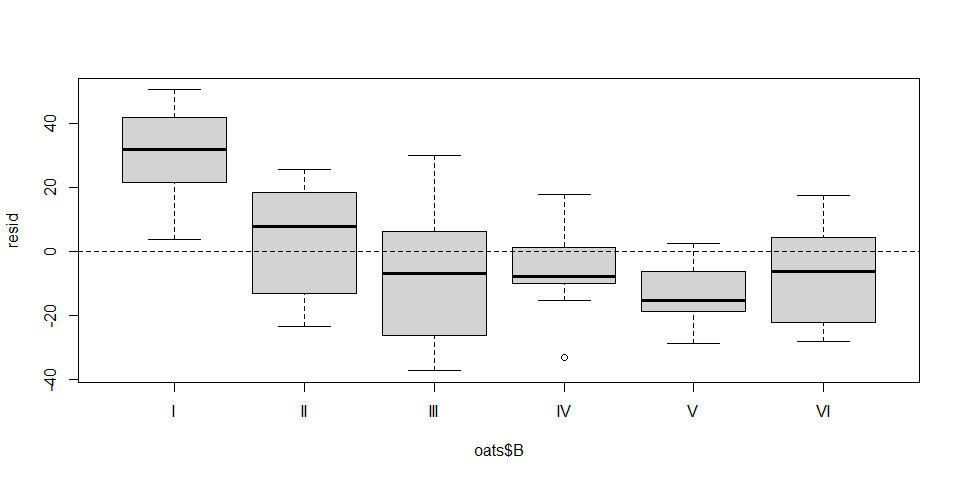
\includegraphics{PractCasa03-full_files/figure-latex/unnamed-chunk-3-1.pdf}

\begin{Shaded}
\begin{Highlighting}[]
\CommentTok{\# Gráfico de Densidad:}
\FunctionTok{plot}\NormalTok{(}\FunctionTok{density}\NormalTok{(ratones}\SpecialCharTok{$}\NormalTok{peso), }\AttributeTok{main =} \StringTok{"Peso ratones"}\NormalTok{)}
\end{Highlighting}
\end{Shaded}

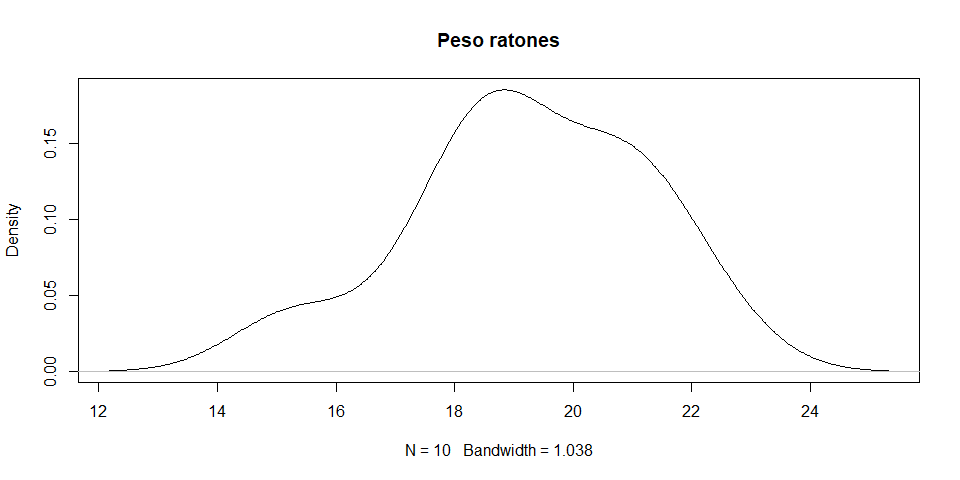
\includegraphics{PractCasa03-full_files/figure-latex/unnamed-chunk-3-2.pdf}

\begin{Shaded}
\begin{Highlighting}[]
\CommentTok{\# Ejecuta un test de normalidad con los datos:}
\FunctionTok{shapiro.test}\NormalTok{(ratones}\SpecialCharTok{$}\NormalTok{peso)}
\end{Highlighting}
\end{Shaded}

\begin{verbatim}
## 
##  Shapiro-Wilk normality test
## 
## data:  ratones$peso
## W = 0.9526, p-value = 0.6993
\end{verbatim}

\begin{Shaded}
\begin{Highlighting}[]
\CommentTok{\# Verifica la simetría y curtosis del conjunto de datos:}
\FunctionTok{library}\NormalTok{(moments)}
\FunctionTok{skewness}\NormalTok{(ratones}\SpecialCharTok{$}\NormalTok{peso)}
\end{Highlighting}
\end{Shaded}

\begin{verbatim}
## [1] -0.4288947
\end{verbatim}

\begin{Shaded}
\begin{Highlighting}[]
\FunctionTok{kurtosis}\NormalTok{(ratones}\SpecialCharTok{$}\NormalTok{peso)}
\end{Highlighting}
\end{Shaded}

\begin{verbatim}
## [1] 2.669256
\end{verbatim}

\begin{Shaded}
\begin{Highlighting}[]
\CommentTok{\# Crea un gráfico Q{-}Q Plot}
\FunctionTok{qqnorm}\NormalTok{(ratones}\SpecialCharTok{$}\NormalTok{peso)}
\FunctionTok{qqline}\NormalTok{(ratones}\SpecialCharTok{$}\NormalTok{peso)}
\end{Highlighting}
\end{Shaded}

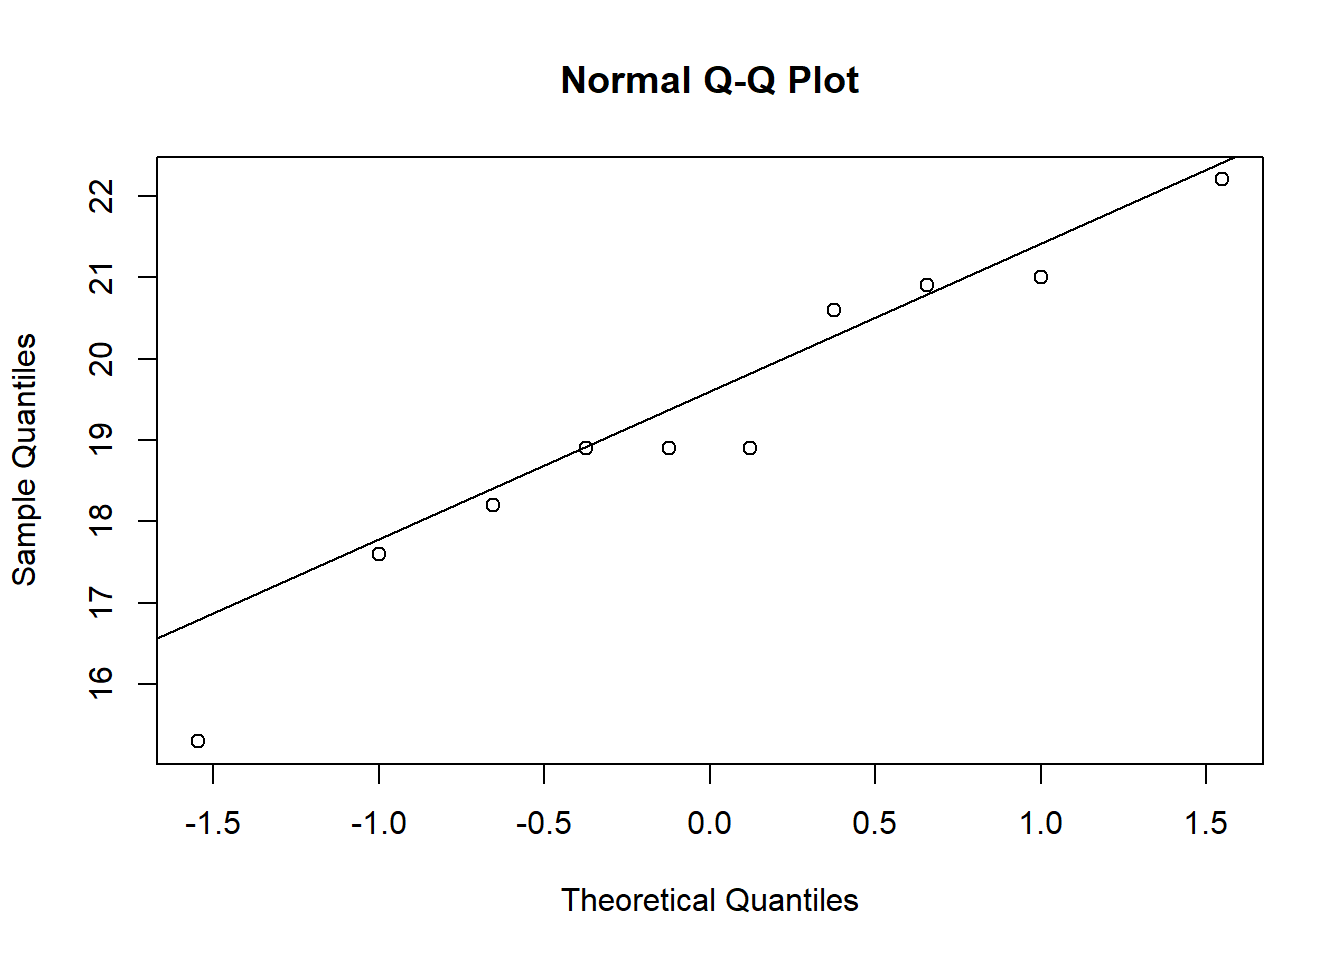
\includegraphics{PractCasa03-full_files/figure-latex/unnamed-chunk-3-3.pdf}

\textbf{Sección de aprendizaje}\\
Ahora aprenderás a realizar un Q-Q Plot más rápido con la función
qqPlot() de la libraría car. Instala la librería car desde el panel
Packages/Install o ejecutándo el siguiente código:

\begin{Shaded}
\begin{Highlighting}[]
\FunctionTok{install.packages}\NormalTok{(}\StringTok{"car"}\NormalTok{)}
\end{Highlighting}
\end{Shaded}

\begin{Shaded}
\begin{Highlighting}[]
\CommentTok{\# Activa la librería car}
\FunctionTok{library}\NormalTok{(car)}

\CommentTok{\# Crea el qqPlot() de la base de datos ratones$peso}
\FunctionTok{qqPlot}\NormalTok{(ratones}\SpecialCharTok{$}\NormalTok{peso)}
\end{Highlighting}
\end{Shaded}

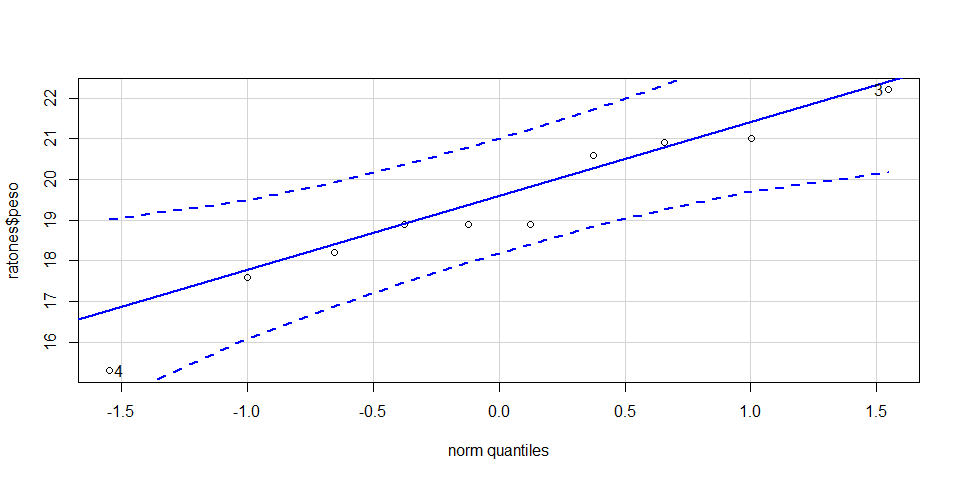
\includegraphics{PractCasa03-full_files/figure-latex/unnamed-chunk-5-1.pdf}

\begin{verbatim}
## [1] 4 3
\end{verbatim}

\textbf{Continua con el Ejercicio 1:}

\begin{Shaded}
\begin{Highlighting}[]
\CommentTok{\# Test 1: Averigua si el promedio de peso de los ratones evaluados}
\CommentTok{\# difiere significativamente de 25 gr (prueba de dos colas)}
\FunctionTok{t.test}\NormalTok{(ratones}\SpecialCharTok{$}\NormalTok{peso, }\AttributeTok{mu =} \DecValTok{26}\NormalTok{, }\AttributeTok{alternative =} \StringTok{"two.sided"}\NormalTok{)}
\end{Highlighting}
\end{Shaded}

\begin{verbatim}
## 
##  One Sample t-test
## 
## data:  ratones$peso
## t = -10.657, df = 9, p-value = 2.102e-06
## alternative hypothesis: true mean is not equal to 26
## 95 percent confidence interval:
##  17.8172 20.6828
## sample estimates:
## mean of x 
##     19.25
\end{verbatim}

\begin{Shaded}
\begin{Highlighting}[]
\CommentTok{\# Test 2: Averigua si el promedio de peso de los ratones evaluados}
\CommentTok{\# es significativamente menor que 25 gr (prueba de una colas)}
\FunctionTok{t.test}\NormalTok{(ratones}\SpecialCharTok{$}\NormalTok{peso, }\AttributeTok{mu =} \DecValTok{26}\NormalTok{, }\AttributeTok{alternative =} \StringTok{"less"}\NormalTok{)}
\end{Highlighting}
\end{Shaded}

\begin{verbatim}
## 
##  One Sample t-test
## 
## data:  ratones$peso
## t = -10.657, df = 9, p-value = 1.051e-06
## alternative hypothesis: true mean is less than 26
## 95 percent confidence interval:
##      -Inf 20.41105
## sample estimates:
## mean of x 
##     19.25
\end{verbatim}

\begin{Shaded}
\begin{Highlighting}[]
\CommentTok{\# Test 3: Averigua si el promedio de peso de los ratones evaluados}
\CommentTok{\# es significativamente mayor que 25 gr (prueba de una colas)}
\FunctionTok{t.test}\NormalTok{(ratones}\SpecialCharTok{$}\NormalTok{peso, }\AttributeTok{mu =} \DecValTok{26}\NormalTok{, }\AttributeTok{alternative =} \StringTok{"greater"}\NormalTok{)}
\end{Highlighting}
\end{Shaded}

\begin{verbatim}
## 
##  One Sample t-test
## 
## data:  ratones$peso
## t = -10.657, df = 9, p-value = 1
## alternative hypothesis: true mean is greater than 26
## 95 percent confidence interval:
##  18.08895      Inf
## sample estimates:
## mean of x 
##     19.25
\end{verbatim}

\hypertarget{ejercicio-2-comparaciones-de-dos-muestras}{%
\section{\texorpdfstring{\textbf{Ejercicio 2: Comparaciones de dos
muestras}}{Ejercicio 2: Comparaciones de dos muestras}}\label{ejercicio-2-comparaciones-de-dos-muestras}}

En un estudio, se han evaluado el efecto de 2 drogas (Columna
\texttt{Droga}, valores A y B) en 8 pacientes y se pretende conocer:

\begin{enumerate}
\def\labelenumi{\arabic{enumi}.}
\item
  si existen diferencias significativas entre el conjunto de datos de la
  droga A y el conjunto de la droga B.
\item
  si el promedio del grupo A es significativamente mayor al promedio del
  grupo B.
\item
  si el promedio del grupo A es significativamente menor al promedio del
  grupo B.
\end{enumerate}

Debes realizar tres test de T. Da un vistazo a los datos para decidir
cual test debes realizar en base a la independencia de los datos o
diferencia de varianza.

Carga el excel \texttt{glicolipido.xlsx} y asígnale el nombre
\texttt{glico}.

Desarrolla lo siguiente:

\begin{Shaded}
\begin{Highlighting}[]
\CommentTok{\# Carga el excel glicolipido.xlsx y asígnale el nombre glico.}
\NormalTok{glico }\OtherTok{\textless{}{-}}\NormalTok{ openxlsx}\SpecialCharTok{::}\FunctionTok{read.xlsx}\NormalTok{(}\StringTok{"\textasciitilde{}}\SpecialCharTok{\textbackslash{}\textbackslash{}}\StringTok{Proyectos\_R}\SpecialCharTok{\textbackslash{}\textbackslash{}}\StringTok{2021}\SpecialCharTok{\textbackslash{}\textbackslash{}}\StringTok{R Data Science}\SpecialCharTok{\textbackslash{}\textbackslash{}}\StringTok{C2{-}S2}\SpecialCharTok{\textbackslash{}\textbackslash{}}\StringTok{glicolipido.xlsx"}\NormalTok{)}

\CommentTok{\# Realiza el boxplot para cada droga}
\FunctionTok{boxplot}\NormalTok{(Glicolipido}\SpecialCharTok{\textasciitilde{}}\NormalTok{Droga, }\AttributeTok{data=}\NormalTok{glico)}
\end{Highlighting}
\end{Shaded}

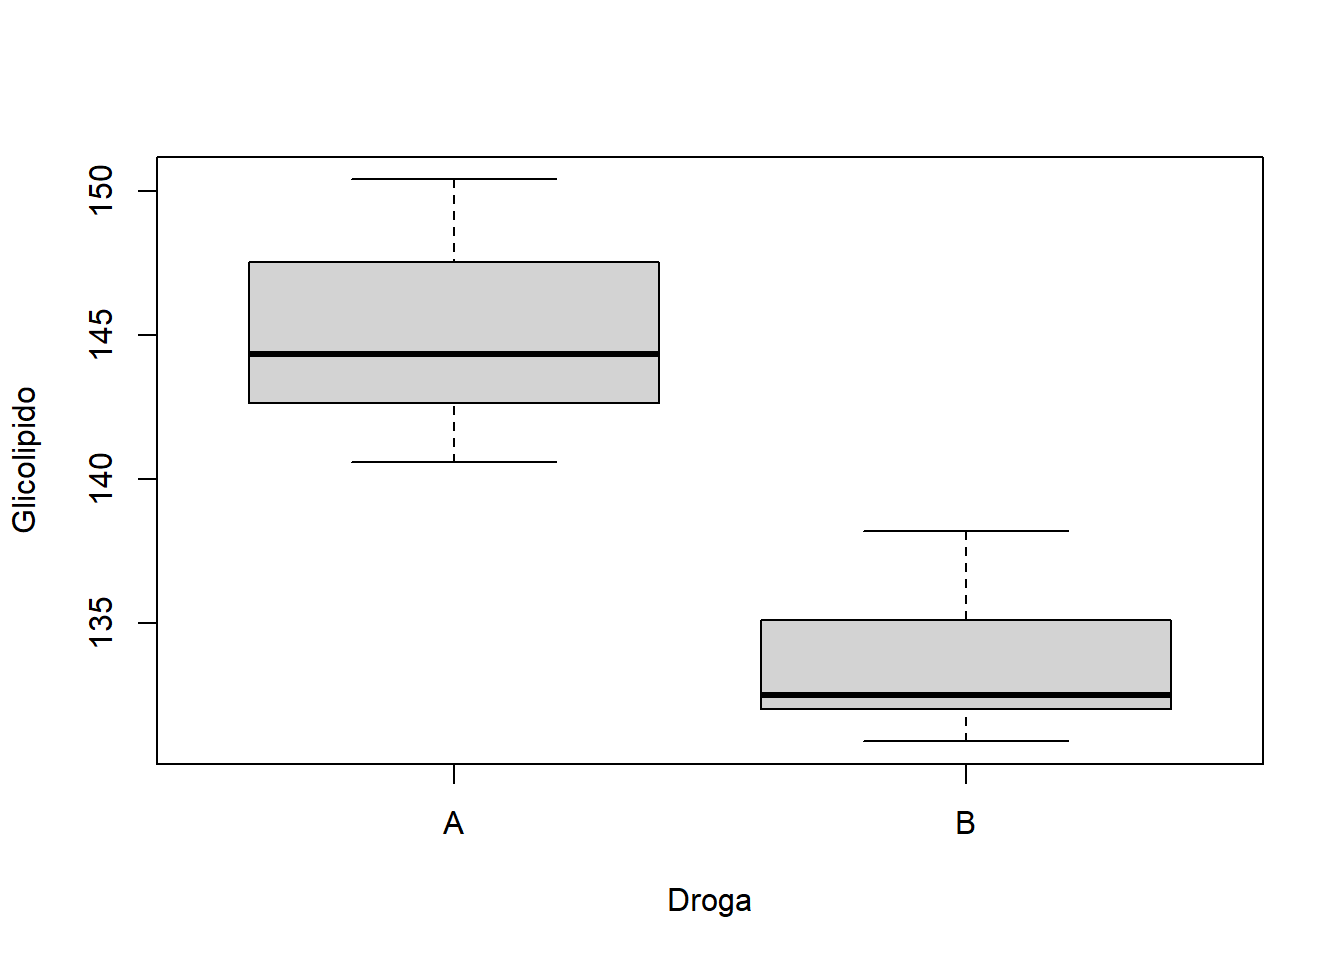
\includegraphics{PractCasa03-full_files/figure-latex/unnamed-chunk-7-1.pdf}

\begin{Shaded}
\begin{Highlighting}[]
\CommentTok{\# Test 1: averigua si existen diferencias significativas entre el conjunto de datos de la droga A y el conjunto de la droga B}
\FunctionTok{t.test}\NormalTok{(Glicolipido }\SpecialCharTok{\textasciitilde{}}\NormalTok{ Droga, }\AttributeTok{data =}\NormalTok{ glico, }\AttributeTok{paired =} \ConstantTok{TRUE}\NormalTok{)}
\end{Highlighting}
\end{Shaded}

\begin{verbatim}
## 
##  Paired t-test
## 
## data:  Glicolipido by Droga
## t = 5.9368, df = 7, p-value = 0.0005777
## alternative hypothesis: true difference in means is not equal to 0
## 95 percent confidence interval:
##   6.904491 16.045509
## sample estimates:
## mean of the differences 
##                  11.475
\end{verbatim}

\begin{Shaded}
\begin{Highlighting}[]
\CommentTok{\# Test 2: averigua si el promedio del grupo A es significativamente mayor al promedio del grupo B}
\FunctionTok{t.test}\NormalTok{(Glicolipido }\SpecialCharTok{\textasciitilde{}}\NormalTok{ Droga, }\AttributeTok{data =}\NormalTok{ glico, }
       \AttributeTok{paired =} \ConstantTok{TRUE}\NormalTok{, }\AttributeTok{alternative =} \StringTok{"greater"}\NormalTok{)}
\end{Highlighting}
\end{Shaded}

\begin{verbatim}
## 
##  Paired t-test
## 
## data:  Glicolipido by Droga
## t = 5.9368, df = 7, p-value = 0.0002888
## alternative hypothesis: true difference in means is greater than 0
## 95 percent confidence interval:
##  7.813028      Inf
## sample estimates:
## mean of the differences 
##                  11.475
\end{verbatim}

\begin{Shaded}
\begin{Highlighting}[]
\CommentTok{\# Test 3: averigua si el promedio del grupo A es significativamente menor al promedio del grupo B.}
\FunctionTok{t.test}\NormalTok{(Glicolipido }\SpecialCharTok{\textasciitilde{}}\NormalTok{ Droga, }\AttributeTok{data =}\NormalTok{ glico, }
       \AttributeTok{paired =} \ConstantTok{TRUE}\NormalTok{, }\AttributeTok{alternative =} \StringTok{"less"}\NormalTok{)}
\end{Highlighting}
\end{Shaded}

\begin{verbatim}
## 
##  Paired t-test
## 
## data:  Glicolipido by Droga
## t = 5.9368, df = 7, p-value = 0.9997
## alternative hypothesis: true difference in means is less than 0
## 95 percent confidence interval:
##      -Inf 15.13697
## sample estimates:
## mean of the differences 
##                  11.475
\end{verbatim}

\hypertarget{ejercicio-3-comparaciones-de-dos-muestras}{%
\section{\texorpdfstring{\textbf{Ejercicio 3: Comparaciones de dos
muestras}}{Ejercicio 3: Comparaciones de dos muestras}}\label{ejercicio-3-comparaciones-de-dos-muestras}}

Siguiendo con la misma base de datos anterior, verifica si existen
diferencias estadísticas entre los sexos para la medición de glicolipido
(columna Glicolipido). Comprueba:

\begin{enumerate}
\def\labelenumi{\arabic{enumi}.}
\item
  si existen diferencias significativas entre el conjunto de datos sexo
  Hombre y el conjunto sexo Mujer.
\item
  si el promedio del sexo Hombre es significativamente mayor al promedio
  del sexo Mujer.
\item
  si el promedio del sexo Hombre es significativamente menor al promedio
  del sexo Mujer.
\end{enumerate}

Debes realizar tres test de T. Da un vistazo a los datos para decidir
cual test debes realizar en base a la independencia de los datos o
diferencia de varianza.

\begin{Shaded}
\begin{Highlighting}[]
\CommentTok{\# Test 1: averigua si existen diferencias significativas entre el conjunto sexo Hombre y el conjunto sexo Mujer}
\FunctionTok{t.test}\NormalTok{(Glicolipido }\SpecialCharTok{\textasciitilde{}}\NormalTok{ Sexo, }\AttributeTok{data =}\NormalTok{ glico, }\AttributeTok{paired =} \ConstantTok{TRUE}\NormalTok{)}
\end{Highlighting}
\end{Shaded}

\begin{verbatim}
## 
##  Paired t-test
## 
## data:  Glicolipido by Sexo
## t = -0.67495, df = 7, p-value = 0.5214
## alternative hypothesis: true difference in means is not equal to 0
## 95 percent confidence interval:
##  -2.139111  1.189111
## sample estimates:
## mean of the differences 
##                  -0.475
\end{verbatim}

\begin{Shaded}
\begin{Highlighting}[]
\CommentTok{\# Test 2: averigua si el promedio del sexo Hombre es significativamente mayor al promedio del sexo Mujer}
\FunctionTok{t.test}\NormalTok{(Glicolipido }\SpecialCharTok{\textasciitilde{}}\NormalTok{ Sexo, }\AttributeTok{data =}\NormalTok{ glico, }
       \AttributeTok{paired =} \ConstantTok{TRUE}\NormalTok{, }\AttributeTok{alternative =} \StringTok{"greater"}\NormalTok{)}
\end{Highlighting}
\end{Shaded}

\begin{verbatim}
## 
##  Paired t-test
## 
## data:  Glicolipido by Sexo
## t = -0.67495, df = 7, p-value = 0.7393
## alternative hypothesis: true difference in means is greater than 0
## 95 percent confidence interval:
##  -1.808315       Inf
## sample estimates:
## mean of the differences 
##                  -0.475
\end{verbatim}

\begin{Shaded}
\begin{Highlighting}[]
\CommentTok{\# Test 3: averigua si el promedio del sexo Hombre es significativamente menor al promedio del sexo Mujer}
\FunctionTok{t.test}\NormalTok{(Glicolipido }\SpecialCharTok{\textasciitilde{}}\NormalTok{ Sexo, }\AttributeTok{data =}\NormalTok{ glico, }
       \AttributeTok{paired =} \ConstantTok{TRUE}\NormalTok{, }\AttributeTok{alternative =} \StringTok{"less"}\NormalTok{)}
\end{Highlighting}
\end{Shaded}

\begin{verbatim}
## 
##  Paired t-test
## 
## data:  Glicolipido by Sexo
## t = -0.67495, df = 7, p-value = 0.2607
## alternative hypothesis: true difference in means is less than 0
## 95 percent confidence interval:
##       -Inf 0.8583148
## sample estimates:
## mean of the differences 
##                  -0.475
\end{verbatim}

\hypertarget{ejercicio-4-lm}{%
\section{\texorpdfstring{\textbf{Ejercicio 4:
LM}}{Ejercicio 4: LM}}\label{ejercicio-4-lm}}

Un estudio de la microbiota del suelo de una región trató de averiguar
cuánto varía la concentración de nitrógeno disponible en el suelo
(columna \texttt{conc.N}) en relación a la cantidad de colonias de
bacterias nitrificantes (columna \texttt{colonias}) halladas en las
muestras obtenidas de la siembra estandarizada en placas petri.

Carga el excel \texttt{suelos.xlsx} y asígnale el nombre
\texttt{suelos}.

\hypertarget{parte-1-modelos-lineales-simples}{%
\subsubsection{\texorpdfstring{\textbf{Parte 1: Modelos lineales
simples}}{Parte 1: Modelos lineales simples}}\label{parte-1-modelos-lineales-simples}}

Desarrolla lo siguiente:

\begin{Shaded}
\begin{Highlighting}[]
\CommentTok{\# Carga el excel suelos.xlsx y asígnale el nombre suelos.}
\NormalTok{suelos }\OtherTok{\textless{}{-}}\NormalTok{  openxlsx}\SpecialCharTok{::}\FunctionTok{read.xlsx}\NormalTok{(}\StringTok{"\textasciitilde{}}\SpecialCharTok{\textbackslash{}\textbackslash{}}\StringTok{Proyectos\_R}\SpecialCharTok{\textbackslash{}\textbackslash{}}\StringTok{2021}\SpecialCharTok{\textbackslash{}\textbackslash{}}\StringTok{R Data Science}\SpecialCharTok{\textbackslash{}\textbackslash{}}\StringTok{C2{-}S2}\SpecialCharTok{\textbackslash{}\textbackslash{}}\StringTok{suelos.xlsx"}\NormalTok{)}

\CommentTok{\# Búsqueda de outliers con boxplot}
\FunctionTok{boxplot}\NormalTok{(suelos}\SpecialCharTok{$}\NormalTok{conc.N)}
\end{Highlighting}
\end{Shaded}

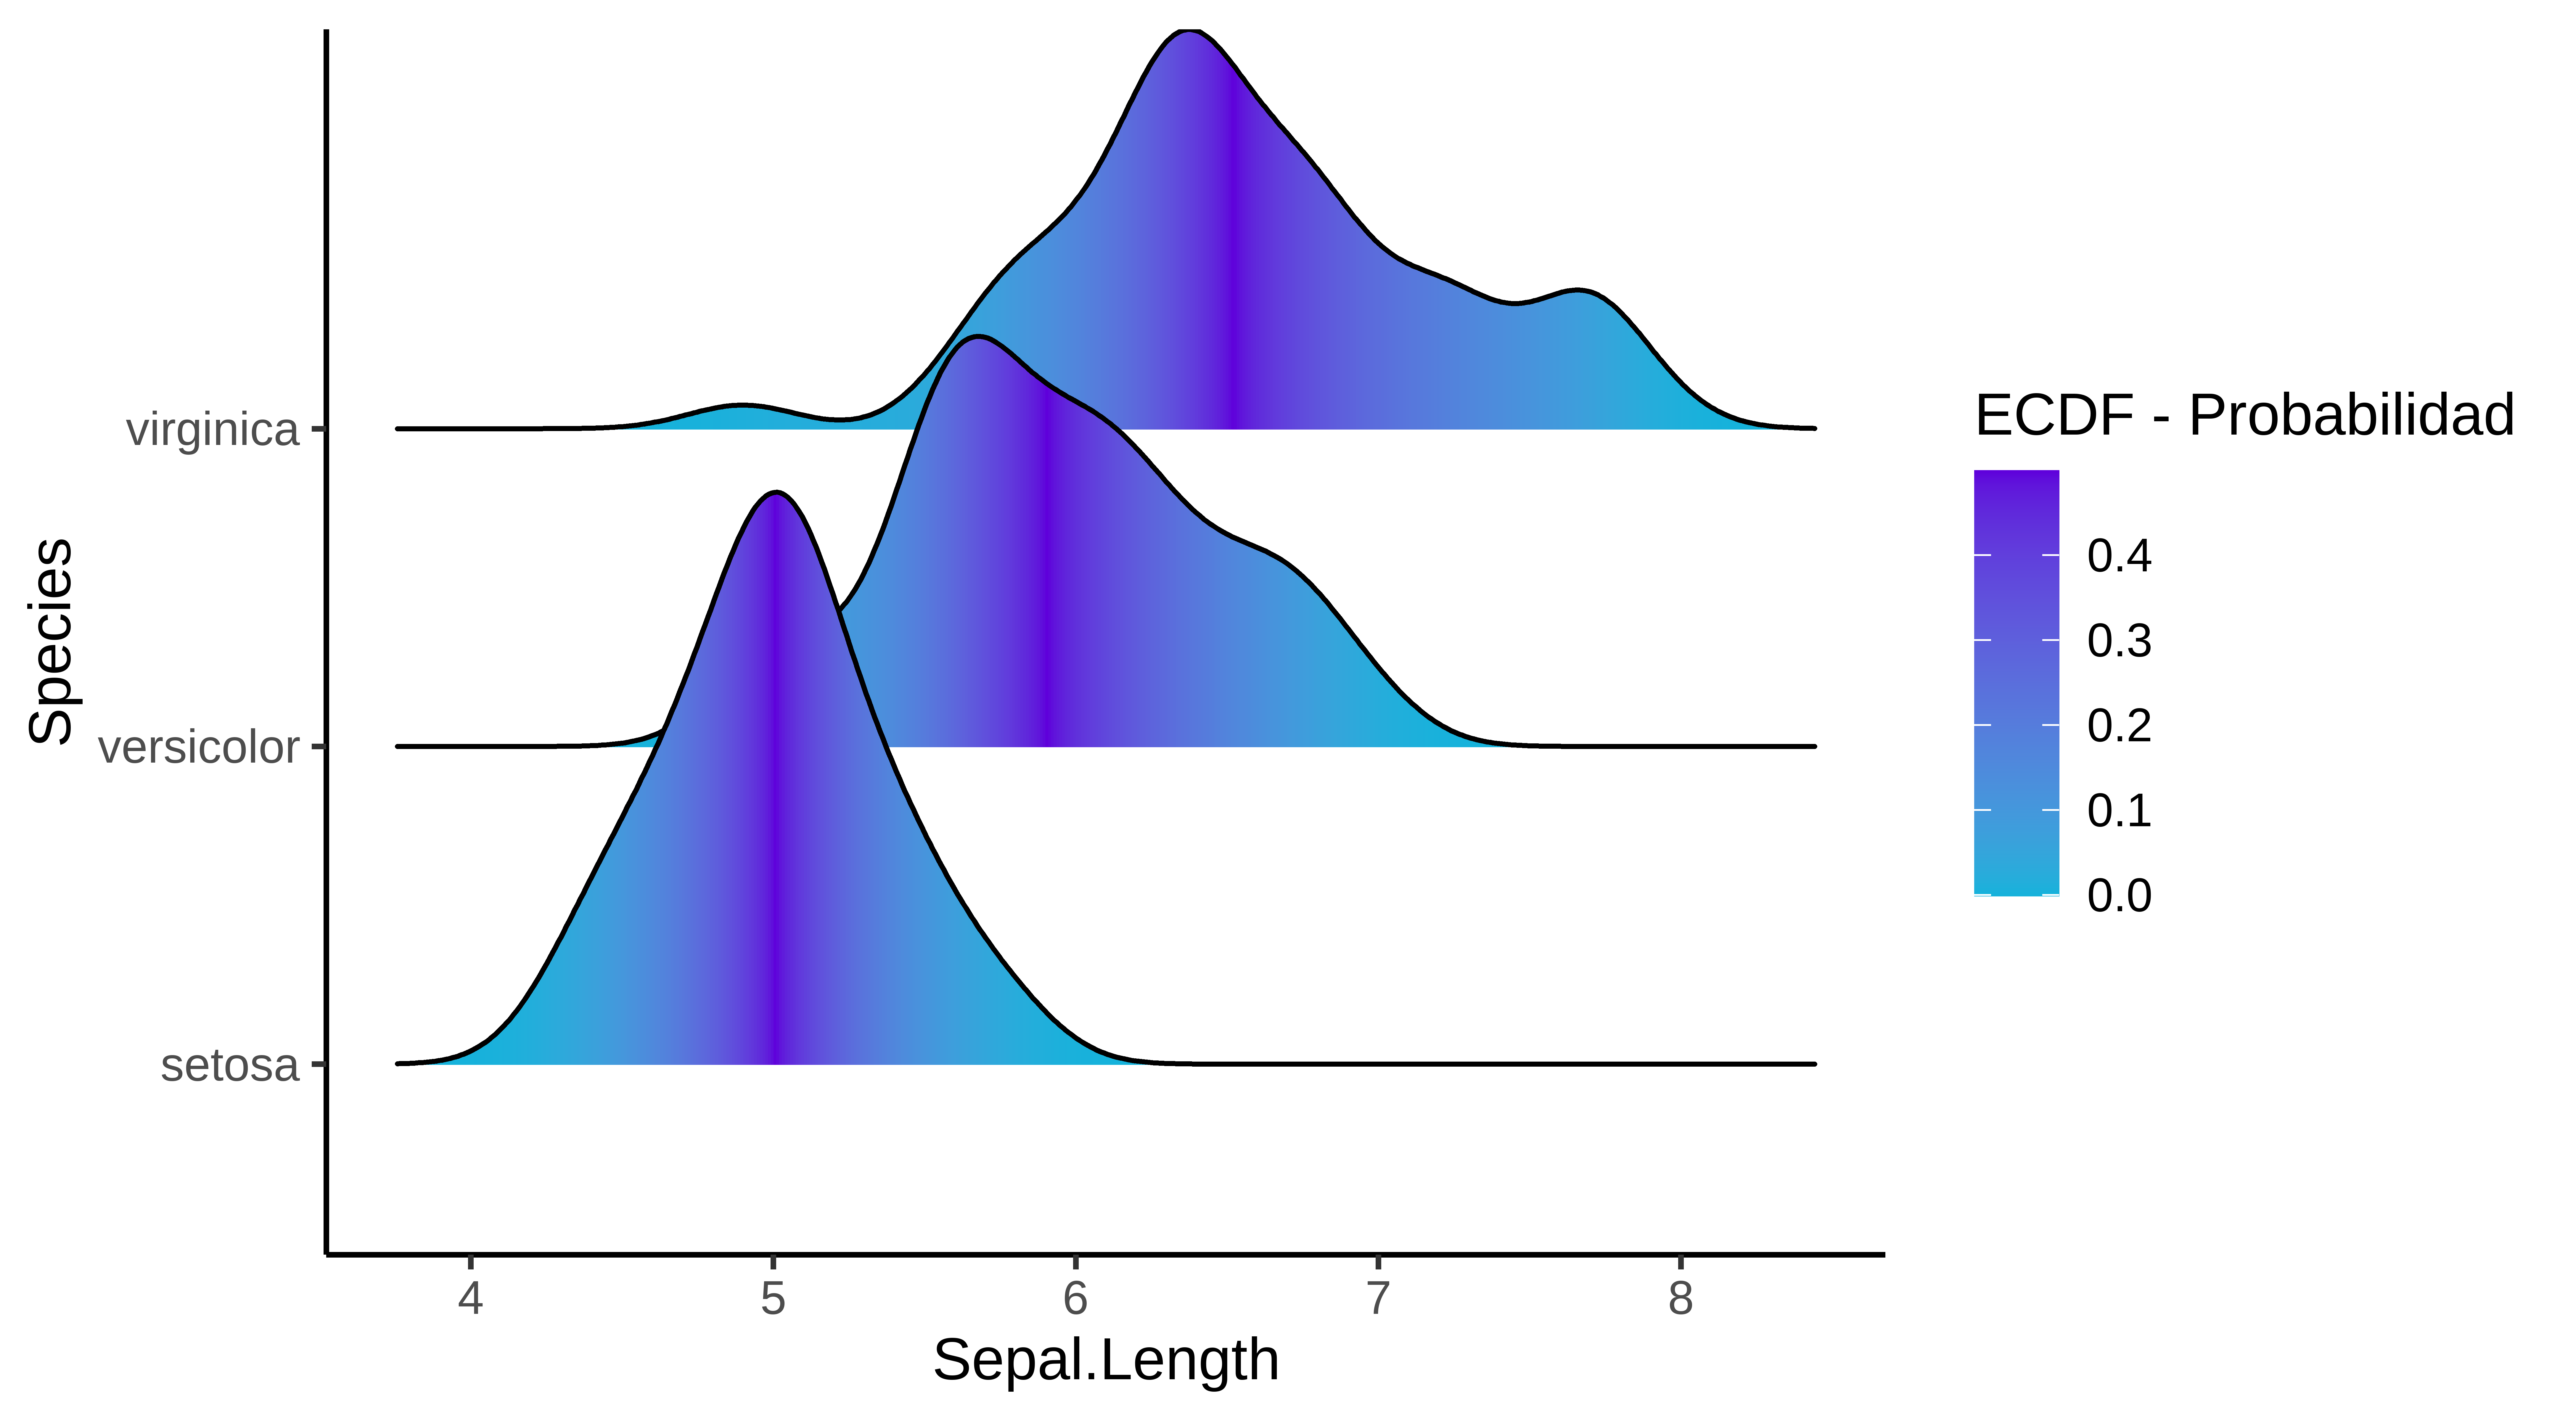
\includegraphics{PractCasa03-full_files/figure-latex/unnamed-chunk-9-1.pdf}

\begin{Shaded}
\begin{Highlighting}[]
\FunctionTok{boxplot.stats}\NormalTok{(suelos}\SpecialCharTok{$}\NormalTok{conc.N)}\SpecialCharTok{$}\NormalTok{out}
\end{Highlighting}
\end{Shaded}

\begin{verbatim}
## [1] 70 50
\end{verbatim}

\begin{Shaded}
\begin{Highlighting}[]
\CommentTok{\# Eliminación de outliers}
\NormalTok{outliers  }\OtherTok{\textless{}{-}} \FunctionTok{identify\_outliers}\NormalTok{(suelos, conc.N)}
\NormalTok{sinOutliers }\OtherTok{\textless{}{-}} \FunctionTok{anti\_join}\NormalTok{(suelos, outliers) }
\end{Highlighting}
\end{Shaded}

\begin{verbatim}
## Joining, by = c("conc.N", "colonias", "plant.simbio", "div.esp.descomp")
\end{verbatim}

\begin{Shaded}
\begin{Highlighting}[]
\CommentTok{\# Verificando que suelos ya no contiene outliers}
\FunctionTok{boxplot}\NormalTok{(sinOutliers}\SpecialCharTok{$}\NormalTok{conc.N)}
\end{Highlighting}
\end{Shaded}

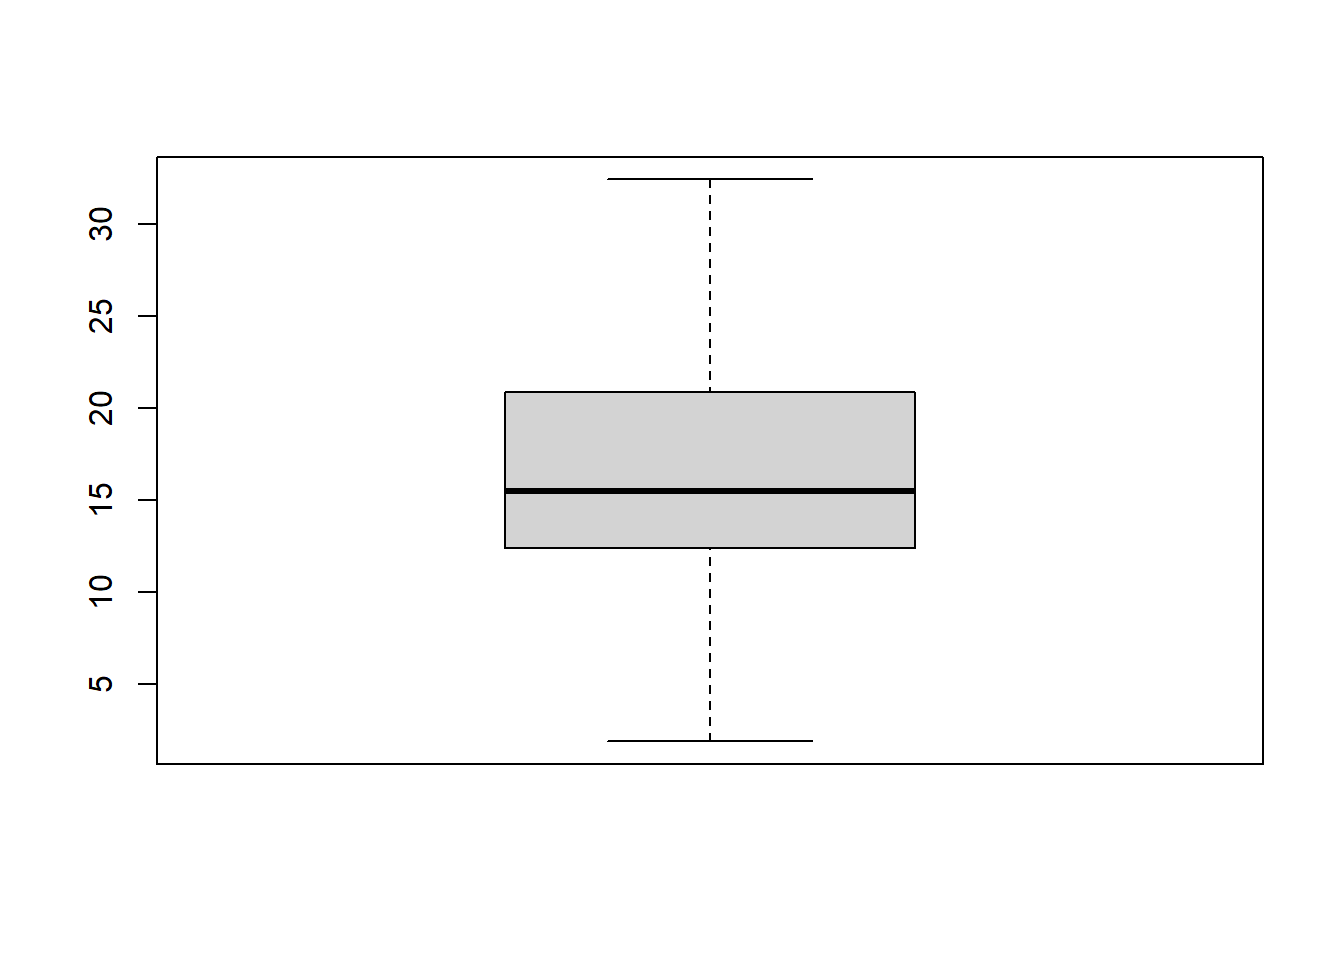
\includegraphics{PractCasa03-full_files/figure-latex/unnamed-chunk-9-2.pdf}

\begin{Shaded}
\begin{Highlighting}[]
\CommentTok{\# Verifica linearidad de las variables respuesta y explicativa}
\FunctionTok{names}\NormalTok{(sinOutliers)}
\end{Highlighting}
\end{Shaded}

\begin{verbatim}
## [1] "conc.N"          "colonias"        "plant.simbio"    "div.esp.descomp"
\end{verbatim}

\begin{Shaded}
\begin{Highlighting}[]
\FunctionTok{plot}\NormalTok{(conc.N}\SpecialCharTok{\textasciitilde{}}\NormalTok{colonias, }\AttributeTok{data=}\NormalTok{sinOutliers)}
\end{Highlighting}
\end{Shaded}

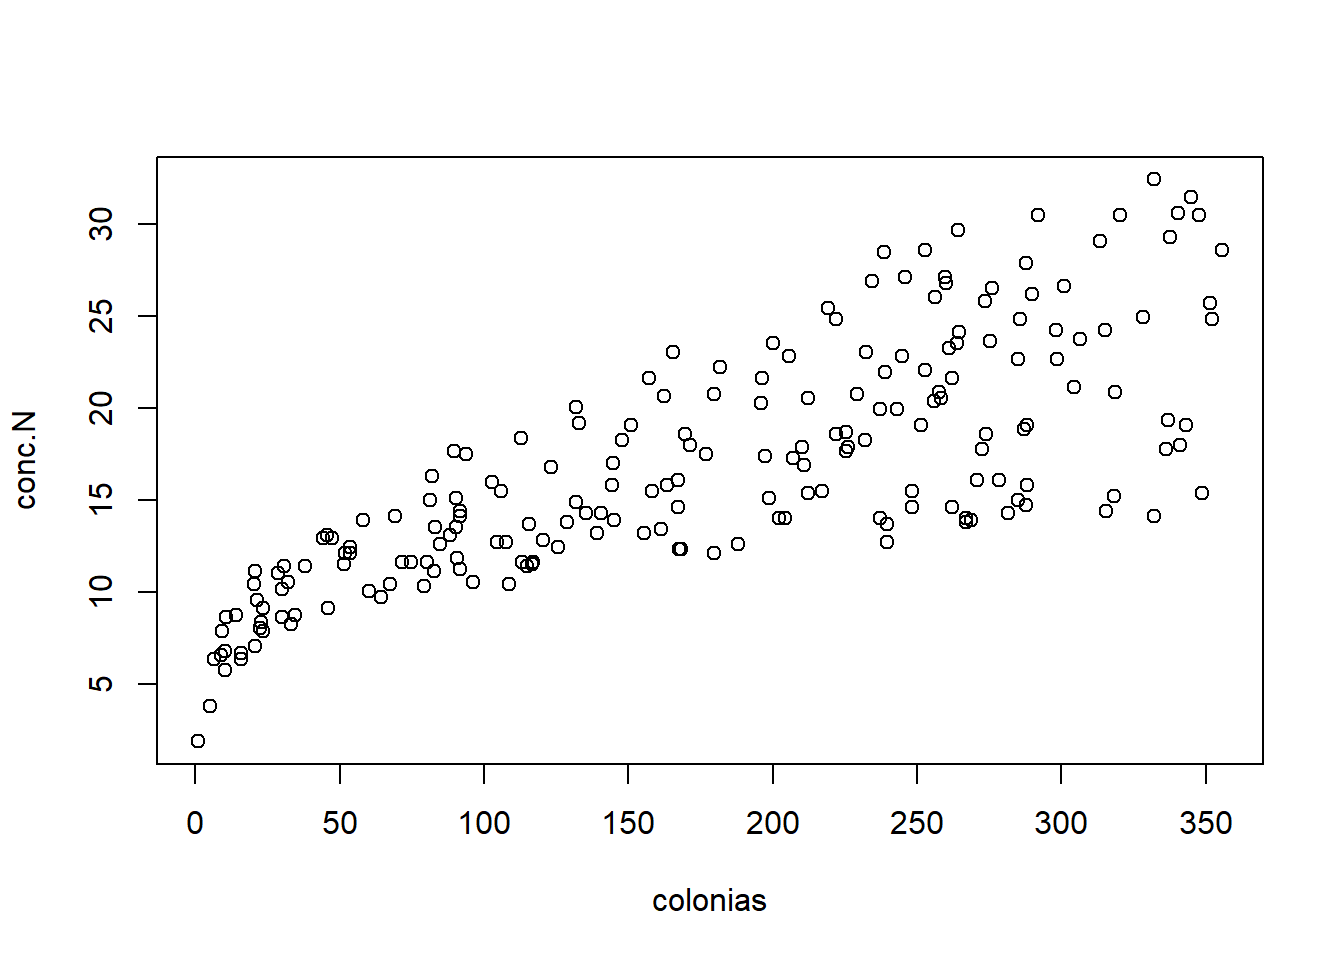
\includegraphics{PractCasa03-full_files/figure-latex/unnamed-chunk-9-3.pdf}

\begin{Shaded}
\begin{Highlighting}[]
\CommentTok{\# Realiza el modelo}
\NormalTok{modelo }\OtherTok{\textless{}{-}} \FunctionTok{lm}\NormalTok{(conc.N}\SpecialCharTok{\textasciitilde{}}\NormalTok{colonias, }\AttributeTok{data=}\NormalTok{sinOutliers)}

\CommentTok{\# Verifica las asunciones teóricas restantes}
\FunctionTok{par}\NormalTok{(}\AttributeTok{mfrow=}\FunctionTok{c}\NormalTok{(}\DecValTok{2}\NormalTok{,}\DecValTok{2}\NormalTok{))}
\FunctionTok{plot}\NormalTok{(modelo)}
\end{Highlighting}
\end{Shaded}

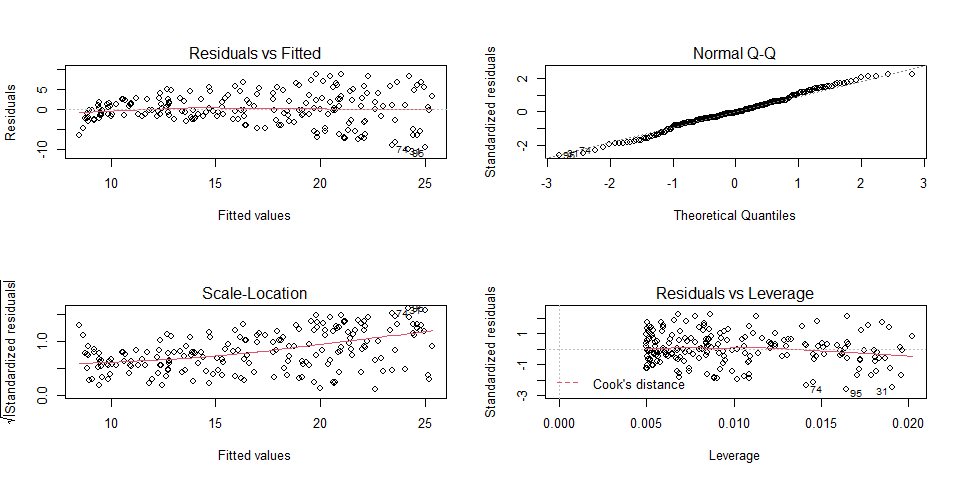
\includegraphics{PractCasa03-full_files/figure-latex/unnamed-chunk-9-4.pdf}

\begin{Shaded}
\begin{Highlighting}[]
\FunctionTok{dev.off}\NormalTok{() }\CommentTok{\#usa siempre dev.off() luego de par() para evitar que siga activo}
\end{Highlighting}
\end{Shaded}

\begin{verbatim}
## null device 
##           1
\end{verbatim}

\begin{Shaded}
\begin{Highlighting}[]
\CommentTok{\# Comprueba la normalidad de los residuales, obtenidos con la función resid()}
\NormalTok{nortest}\SpecialCharTok{::}\FunctionTok{ad.test}\NormalTok{(}\FunctionTok{resid}\NormalTok{(modelo))}
\end{Highlighting}
\end{Shaded}

\begin{verbatim}
## 
##  Anderson-Darling normality test
## 
## data:  resid(modelo)
## A = 0.49121, p-value = 0.217
\end{verbatim}

\begin{Shaded}
\begin{Highlighting}[]
\NormalTok{moments}\SpecialCharTok{::}\FunctionTok{skewness}\NormalTok{(}\FunctionTok{resid}\NormalTok{(modelo))}
\end{Highlighting}
\end{Shaded}

\begin{verbatim}
## [1] -0.08863202
\end{verbatim}

\begin{Shaded}
\begin{Highlighting}[]
\NormalTok{moments}\SpecialCharTok{::}\FunctionTok{kurtosis}\NormalTok{(}\FunctionTok{resid}\NormalTok{(modelo))}
\end{Highlighting}
\end{Shaded}

\begin{verbatim}
## [1] 2.779015
\end{verbatim}

\begin{Shaded}
\begin{Highlighting}[]
\FunctionTok{plot}\NormalTok{(}\FunctionTok{density}\NormalTok{(}\FunctionTok{resid}\NormalTok{(modelo)))}

\CommentTok{\# Obtén los resultados del modelo e interprétalo}
\FunctionTok{summary}\NormalTok{(modelo)}
\end{Highlighting}
\end{Shaded}

\begin{verbatim}
## 
## Call:
## lm(formula = conc.N ~ colonias, data = sinOutliers)
## 
## Residuals:
##      Min       1Q   Median       3Q      Max 
## -10.0632  -2.3454  -0.2295   2.4805   8.6548 
## 
## Coefficients:
##             Estimate Std. Error t value Pr(>|t|)    
## (Intercept) 8.439112   0.549412   15.36   <2e-16 ***
## colonias    0.047537   0.002691   17.67   <2e-16 ***
## ---
## Signif. codes:  0 '***' 0.001 '**' 0.01 '*' 0.05 '.' 0.1 ' ' 1
## 
## Residual standard error: 3.91 on 198 degrees of freedom
## Multiple R-squared:  0.6119, Adjusted R-squared:  0.6099 
## F-statistic: 312.1 on 1 and 198 DF,  p-value: < 2.2e-16
\end{verbatim}

\textbf{Interpreta los resultados de la regresión y responde:}

\textbf{P1:} \emph{¿El modelo fue significativo?}

\textbf{Rpta/.} Sí, con p-value: \textless{} 2.2e-16, generado a partir
de la prueba F con valor 312.1 y 198 grados de libertad.

\textbf{\hfill\break
P2:} \emph{¿Cuánto aumenta el nitrógeno en relación a las colonias de
bacterias nitrificantes contabilizadas en la muestra?}

\textbf{Rpta/.} Por cada colonia contabilizada en la muestra sembrada en
placa petri, la concentración del nitrógeno en el suelo aumenta en 0.048
unidades.

\textbf{P3:} \emph{¿Cuánta varianza de la variable respuesta es
explicada por la variable respuesta?}

\textbf{Rpta/.} 60.99\%, debido al Adjusted R-squared: 0.6099

\hypertarget{parte-2-modelos-lineales-muxfaltiples-aditivos}{%
\subsubsection{\texorpdfstring{\textbf{Parte 2: Modelos lineales
múltiples
(aditivos)}}{Parte 2: Modelos lineales múltiples (aditivos)}}\label{parte-2-modelos-lineales-muxfaltiples-aditivos}}

Considera incluir en el modelo dos nuevas variables explicativas: un
indice de diversidad de plantas \texttt{plant.simbio} y la diversidad de
especies descomponedoras de materia orgánica \texttt{div.esp.descomp}
como potenciales variables que puedan mejorar el modelo. Crea la
variable \texttt{modelo2} incluyendo dichas nuevas variables y verifica:

\begin{enumerate}
\def\labelenumi{\arabic{enumi}.}
\item
  Si \texttt{modelo2} es significativo.
\item
  Si hay variables que no sean significativas (ver columna
  \texttt{Pr(\textgreater{}\textbar{}t\textbar{})} en el resumen de
  \texttt{summary()}).
\end{enumerate}

\begin{Shaded}
\begin{Highlighting}[]
\FunctionTok{names}\NormalTok{(sinOutliers)}
\end{Highlighting}
\end{Shaded}

\begin{verbatim}
## [1] "conc.N"          "colonias"        "plant.simbio"    "div.esp.descomp"
\end{verbatim}

\begin{Shaded}
\begin{Highlighting}[]
\NormalTok{modelo2 }\OtherTok{\textless{}{-}} \FunctionTok{lm}\NormalTok{(conc.N}\SpecialCharTok{\textasciitilde{}}\NormalTok{colonias}\SpecialCharTok{+}\NormalTok{plant.simbio}\SpecialCharTok{+}\NormalTok{div.esp.descomp, }\AttributeTok{data=}\NormalTok{sinOutliers)}
\NormalTok{modelo2 }\OtherTok{\textless{}{-}} \FunctionTok{lm}\NormalTok{(conc.N}\SpecialCharTok{\textasciitilde{}}\NormalTok{.,}\AttributeTok{data=}\NormalTok{sinOutliers)}
\FunctionTok{summary}\NormalTok{(modelo2)}
\end{Highlighting}
\end{Shaded}

\begin{verbatim}
## 
## Call:
## lm(formula = conc.N ~ ., data = sinOutliers)
## 
## Residuals:
##      Min       1Q   Median       3Q      Max 
## -10.5161  -1.0677   0.2979   1.4510   3.4013 
## 
## Coefficients:
##                  Estimate Std. Error t value Pr(>|t|)    
## (Intercept)      3.565738   0.442005   8.067 7.05e-14 ***
## colonias         0.045751   0.001394  32.824  < 2e-16 ***
## plant.simbio     0.187530   0.008311  22.564  < 2e-16 ***
## div.esp.descomp -0.001294   0.005660  -0.229    0.819    
## ---
## Signif. codes:  0 '***' 0.001 '**' 0.01 '*' 0.05 '.' 0.1 ' ' 1
## 
## Residual standard error: 2.023 on 196 degrees of freedom
## Multiple R-squared:  0.8972, Adjusted R-squared:  0.8956 
## F-statistic: 570.3 on 3 and 196 DF,  p-value: < 2.2e-16
\end{verbatim}

De haber detectado alguna variable explicativa no significativa, esta
debe ser eliminada del modelo ya que le no aportan nada. Por el
contrario, el modelo se beneficia al eliminar variables no
significativas. Crea la variable \texttt{modelo3} que contenga el nuevo
modelo mejorado.

\begin{Shaded}
\begin{Highlighting}[]
\NormalTok{modelo3 }\OtherTok{\textless{}{-}} \FunctionTok{lm}\NormalTok{(conc.N}\SpecialCharTok{\textasciitilde{}}\NormalTok{.,}\AttributeTok{data=}\NormalTok{sinOutliers[,}\SpecialCharTok{{-}}\DecValTok{4}\NormalTok{])}
\FunctionTok{summary}\NormalTok{(modelo3)}
\end{Highlighting}
\end{Shaded}

\begin{verbatim}
## 
## Call:
## lm(formula = conc.N ~ ., data = sinOutliers[, -4])
## 
## Residuals:
##      Min       1Q   Median       3Q      Max 
## -10.5572  -1.0502   0.2906   1.4049   3.3994 
## 
## Coefficients:
##              Estimate Std. Error t value Pr(>|t|)    
## (Intercept)   3.50532    0.35339   9.919   <2e-16 ***
## colonias      0.04575    0.00139  32.909   <2e-16 ***
## plant.simbio  0.18799    0.00804  23.382   <2e-16 ***
## ---
## Signif. codes:  0 '***' 0.001 '**' 0.01 '*' 0.05 '.' 0.1 ' ' 1
## 
## Residual standard error: 2.018 on 197 degrees of freedom
## Multiple R-squared:  0.8972, Adjusted R-squared:  0.8962 
## F-statistic: 859.6 on 2 and 197 DF,  p-value: < 2.2e-16
\end{verbatim}

\textbf{P4:} \emph{¿El modelo muestra alguna mejora respecto a la
cantidad de varianza explicada por las variables independientes
(explicativas)? (comparar R cuadrados ajustados de los modelos 2 y 3)}

\textbf{Rpta/.} Sí se mejoró el modelo al incluir a la variable
plant.simbio, con un R2 ajustado de 0.89, es decir que las variables
explicativas de este modelo explican el 89\% de la varianza de la
variable respuesta \texttt{conc.N}.

\hypertarget{parte-3-interpretaciuxf3n-de-coeficientes-en-modelos-simples-o-muxfaltiples-aditivos}{%
\subsubsection{\texorpdfstring{\textbf{Parte 3: Interpretación de
coeficientes en modelos simples o múltiples
aditivos}}{Parte 3: Interpretación de coeficientes en modelos simples o múltiples aditivos}}\label{parte-3-interpretaciuxf3n-de-coeficientes-en-modelos-simples-o-muxfaltiples-aditivos}}

En consecuencia, podemos leer un modelo simple y aditivo de la siguiente
manera, siendo que la fórmula de una regresión simple es:

\[
y=β0+β1∗x1
\]

y la de una regresión múltiple aditiva con dos variables explicativas
es:

\[
y=β0+β1∗x1+β2∗x2
\]

\textbf{En ambos casos, los coeficientes se leen igual:}

\begin{itemize}
\item
  \textbf{Intercepto (β0):} es el promedio de la variable respuesta y
  cuando la o las variables respuesta son 0 (es decir, sin contar con el
  efecto de la variable explicativa).

  \[
  y=β0+β1∗(0) = β0+0 = β0  
  \]
\end{itemize}

o para las regresiones múltiples aditivas\[
y=β0+β1∗(0)+β2∗(0) = β0+0+0 = β0  
\]

\begin{itemize}
\tightlist
\item
  \textbf{Pendiente de x1 (β1) o x2 (β2):} se interpreta como "el
  aumento de 1 unidad de la variable explicativa x1, representa un
  aumento de β1~en el promedio de la variable respuesta y. Lo mismo para
  x2 y su respectivo aumento β2.
\end{itemize}

\hypertarget{parte-4-modelos-lineales-muxfaltiples-interacciuxf3n}{%
\subsubsection{\texorpdfstring{\textbf{Parte 4: Modelos lineales
múltiples
(interacción)}}{Parte 4: Modelos lineales múltiples (interacción)}}\label{parte-4-modelos-lineales-muxfaltiples-interacciuxf3n}}

Este tipo de modelos se desarrollan cuando uno quiere responder
preguntas del tipo:

\begin{enumerate}
\def\labelenumi{\arabic{enumi}.}
\item
  ¿La variable C modera la relación entre B y A?,
\item
  ¿La fuerza del efecto B y A depende de C?,
\item
  ¿Cómo afecta C a la relación entre B y A? ,
\item
  ¿Cómo influye C en la relación B y A?
\end{enumerate}

Ahora, verifica si es que, adicionalmente a los efectos principales
individuales de las variables, existe algún efecto significativo de la
interacción de las variables respuesta \texttt{colonias} y
\texttt{plant.simbio} que explique algo de la varianza restante de la
variable respuesta \texttt{conc.N}. Para indicar interacciones debes
colocar un símbolo de multiplicación entre las variables que deseas que
interactúen en el modelo.

\begin{Shaded}
\begin{Highlighting}[]
\NormalTok{modelo4 }\OtherTok{\textless{}{-}} \FunctionTok{lm}\NormalTok{(conc.N }\SpecialCharTok{\textasciitilde{}}\NormalTok{ colonias}\SpecialCharTok{*}\NormalTok{plant.simbio, }\AttributeTok{data =}\NormalTok{ sinOutliers)}
\FunctionTok{summary}\NormalTok{(modelo4)}
\end{Highlighting}
\end{Shaded}

\begin{verbatim}
## 
## Call:
## lm(formula = conc.N ~ colonias * plant.simbio, data = sinOutliers)
## 
## Residuals:
##     Min      1Q  Median      3Q     Max 
## -7.6039 -0.4833  0.2197  0.7137  1.8295 
## 
## Coefficients:
##                        Estimate Std. Error t value Pr(>|t|)    
## (Intercept)           8.100e+00  2.974e-01  27.233   <2e-16 ***
## colonias              1.910e-02  1.504e-03  12.699   <2e-16 ***
## plant.simbio          2.886e-02  8.905e-03   3.241   0.0014 ** 
## colonias:plant.simbio 9.054e-04  4.368e-05  20.727   <2e-16 ***
## ---
## Signif. codes:  0 '***' 0.001 '**' 0.01 '*' 0.05 '.' 0.1 ' ' 1
## 
## Residual standard error: 1.132 on 196 degrees of freedom
## Multiple R-squared:  0.9678, Adjusted R-squared:  0.9673 
## F-statistic:  1963 on 3 and 196 DF,  p-value: < 2.2e-16
\end{verbatim}

\hypertarget{parte-5-interpretaciuxf3n-de-coeficientes-en-modelos-lineales-muxfaltiples-interacciuxf3n}{%
\subsubsection{\texorpdfstring{\textbf{Parte 5: Interpretación de
coeficientes en modelos lineales múltiples
(interacción)}}{Parte 5: Interpretación de coeficientes en modelos lineales múltiples (interacción)}}\label{parte-5-interpretaciuxf3n-de-coeficientes-en-modelos-lineales-muxfaltiples-interacciuxf3n}}

Cuando existe un efecto de interacción, el efecto de una variable
explicativa (x1) depende de los valores de una o más variables
explicativas (x2, x3,\ldots).

La interacción en un modelo con interacciones cambia el cómo
interpretamos los resultados. Primero hay que revisar si la interacción
fue significativa. Antes de interpretar, revisemos la fórmula de la
regresión múltiple con interacción:\[
y=b0+b1∗x1+b2∗x2+b3∗x1∗x2
\]

Si factorizamos la fórmula tomando en cuenta x1, tenemos:

\[
y=(b0+b2∗x2)+(b1+b3∗x2)∗x1
\]

Si nos percatamos, esa fórmula se asemeja en estructura a
\(y=b0+b1*x1\), ¿cierto?, significa que de la ecuación anterior,
\((b1+b3∗x2)\) es la pendiente de x1. Es decir, la pendiente de la
variable x1 cambiará por la influencia de la variable x2.

Cuando se realiza una regresión múltiple con interacciones buscamos
interpretar el término de la interacción, por lo que no nos interesa
demasiado el efecto de cada variable respuesta independientemente una de
la otra.

\begin{itemize}
\tightlist
\item
  \underline{El efecto de \texttt{colonias}(la primera variable
  explicativa) es:} \(β1*x1+ β3*x1*x2\)
\end{itemize}

lo que es en nuestro ejemplo: \(β1*colonias + β3*colonias*plant.simbio\)

Reemplazando los valores de la regresión β1 es 0.04575 y β3 es 0.18799,
tenemos: \(0.04575*colonias + 0.18799*colonias*plant.simbio\)

Para interpretar decimos, si la variable \texttt{plant.simbio} es 0 (el
indice de diversidad de plantas simbióticas es 0), entonces
\texttt{conc.N} (la variable respuesta \texttt{y}) se reduce a
\(0.04575*colonias + 0.18799*colonias*0 = 0.04575*colonias\), es decir,
cuando \texttt{plant.simbio} es 0, una unidad de incremento de colonias,
aumenta el promedio esperado de la variable \texttt{conc.N} (y) en
0.04575 unidades.

Para interpretar decimos, si la variable \texttt{plant.simbio} es 1 (el
indice de diversidad de plantas simbióticas es 0), entonces
\texttt{conc.N} (la variable respuesta \texttt{y}) se reduce a
\(0.04575*colonias + 0.18799*colonias*1 = 0.04575*colonias + 0.18799*colonias\),
es decir, cuando \texttt{plant.simbio} es 1, una unidad de incremento de
colonias, incrementa el promedio esperado de la variable \texttt{conc.N}
(y) en 0.04575 + 0.18799 unidades, o 0.23374 unidades.

\begin{itemize}
\item
  De la misma manera podrías interpretar el efecto de
  \texttt{plant.simbio.}
\item
  \textbf{Haciendo una interpretación ``más del mundo real''}, podemos
  decir: la concentración de nitrógeno (\texttt{conc.N}) tiende a ser
  mayor en zonas donde la cantidad de unidades formadoras de colonias
  (\texttt{colonias}) es mayor; sin embargo, esta relación se incrementa
  más cuando los suelos, además de tener mayor abundancia de unidades
  formadoras de colonias, tiene también mayor diversidad de plantas
  simbióticas (\texttt{plant.simbio}). En suma, la fuerza de la relación
  positiva entre \texttt{conc.N} (y) y \texttt{colonias} (x1) depende de
  la presencia de un mayor valor de \texttt{plant.simbio} (x2) en la
  zona de estudios.
\end{itemize}

\begin{quote}
\textbf{Nota final:} Gracias al principio jerárquico en modelos
lineales, si incluimos una interacción en un modelo y es significativa,
no importa si p-valores de los efectos independientes no lo son.
\end{quote}

\hypertarget{ejercicio-5-anova}{%
\section{\texorpdfstring{\textbf{Ejercicio 5:
ANOVA}}{Ejercicio 5: ANOVA}}\label{ejercicio-5-anova}}

Se realizaron mediciones de la longitud total coporal (columna
\texttt{long\_total}) de tres subespecie de la especie Microlophus
thoraccicus, halladas en la costa norte de Peru. Realiza en análisis de
varianza ANOVA para corroborar si existen diferencias entre los grupos.
De hallar diferencias, identifica el grupo que es diferente entre los
tres. Carga el excel sp.xlsx para realizar este ejercicio.

\begin{Shaded}
\begin{Highlighting}[]
\CommentTok{\# Carga el excel sp.xlsx y asígnale el nombre sp}
\NormalTok{sp }\OtherTok{\textless{}{-}}\NormalTok{ openxlsx}\SpecialCharTok{::}\FunctionTok{read.xlsx}\NormalTok{(}\StringTok{"\textasciitilde{}}\SpecialCharTok{\textbackslash{}\textbackslash{}}\StringTok{Proyectos\_R}\SpecialCharTok{\textbackslash{}\textbackslash{}}\StringTok{2021}\SpecialCharTok{\textbackslash{}\textbackslash{}}\StringTok{R Data Science}\SpecialCharTok{\textbackslash{}\textbackslash{}}\StringTok{C2{-}S2}\SpecialCharTok{\textbackslash{}\textbackslash{}}\StringTok{sp.xlsx"}\NormalTok{)}

\CommentTok{\# Elimina outliers}
\NormalTok{out }\OtherTok{\textless{}{-}}\NormalTok{ sp }\SpecialCharTok{\%\textgreater{}\%} 
  \FunctionTok{group\_by}\NormalTok{(ssp) }\SpecialCharTok{\%\textgreater{}\%} 
  \FunctionTok{identify\_outliers}\NormalTok{(long\_total)}

\NormalTok{sp2 }\OtherTok{\textless{}{-}} \FunctionTok{anti\_join}\NormalTok{(sp,out)}

\CommentTok{\# Con la base de datos filtrada, si es que fue necesario,}
\CommentTok{\# analiza qué anova realizarás. Comprueba si se debe }
\CommentTok{\# realizar un anova balanceado o no balanceado.}
\FunctionTok{table}\NormalTok{(sp}\SpecialCharTok{$}\NormalTok{ssp)}

\CommentTok{\# Realiza el modelo lineal y asignalo con le nombre "modelo"}
\NormalTok{modelo  }\OtherTok{\textless{}{-}} \FunctionTok{lm}\NormalTok{(long\_total }\SpecialCharTok{\textasciitilde{}}\NormalTok{ ssp, }\AttributeTok{data =}\NormalTok{ sp)}

\CommentTok{\# Realiza el ANOVA}
\FunctionTok{anova}\NormalTok{(modelo) }

\CommentTok{\# Verifica la normalidad de los residuales}
\FunctionTok{shapiro.test}\NormalTok{(}\FunctionTok{resid}\NormalTok{(modelo))}

\CommentTok{\# Verifica la homogeneidad de varianzas}
\FunctionTok{bartlett.test}\NormalTok{(long\_total }\SpecialCharTok{\textasciitilde{}}\NormalTok{ ssp, }\AttributeTok{data =}\NormalTok{ sp)}

\CommentTok{\# Realiza el Test posthoc respectivo}
\FunctionTok{TukeyHSD}\NormalTok{(}\FunctionTok{aov}\NormalTok{(modelo))}
\end{Highlighting}
\end{Shaded}

\hypertarget{ejercicio-6-balancear-un-anova-una-vuxeda}{%
\section{\texorpdfstring{\textbf{Ejercicio 6: Balancear un ANOVA (una
vía)}}{Ejercicio 6: Balancear un ANOVA (una vía)}}\label{ejercicio-6-balancear-un-anova-una-vuxeda}}

Muchas veces tenemos N muestral suficiente como para uniformizar el
ANOVA. Esta decisión, puede explotar lo mejor del ANOVA balanceado
frente a uno desbalanceado. En general, se asume que los ANOVA
balanceados tienen un mayor poder estadístico, menor susceptibilidad
ante ligeras desviaciones del supuesto de homocedasticidad (igualdad) de
varianzas entre grupos, que lo ANOVA no balanceados. Así que este
procedimiento te ayudará ante aquellas situaciones en las que necesites
balancear.

En el siguiente ejemplo verificaremos si existe diferencias
significativas entre los niveles de la variable explicativa
\texttt{tratamiento}, respecto a la variable respuesta \texttt{y}. Los
niveles de la variable explicativa son 3: Ctrl, trat1 y trat2. Esta base
de datos es desbalanceada. Verifica la presencia de outliers y
elimínalos. Posteriormente, trata de balancear el análisis, eliminando
aleatoriamente filas dentro de los niveles que lo requieran para que
todos tengan la misma cantidad de observaciones. Continua verificando
los supuestos teóricos del ANOVA balanceado y obtén los resultados. Si
el ejercicio lo requiere, realiza un test post hoc para identificar qué
nivel de \texttt{tratamiento} es el que genera un mayor incremento en el
promedio estimado de la variable \texttt{y}.

Carga el excel \texttt{ejercicio\_grupos.xlsx}para comenzar el
ejercicio.

\begin{Shaded}
\begin{Highlighting}[]
\CommentTok{\# Carga el excel ejercicio\_grupos.xlsx y asígnale el nombre grupos}
\NormalTok{grupos }\OtherTok{\textless{}{-}}\NormalTok{ openxlsx}\SpecialCharTok{::}\FunctionTok{read.xlsx}\NormalTok{(}\StringTok{"\textasciitilde{}}\SpecialCharTok{\textbackslash{}\textbackslash{}}\StringTok{Proyectos\_R}\SpecialCharTok{\textbackslash{}\textbackslash{}}\StringTok{2021}\SpecialCharTok{\textbackslash{}\textbackslash{}}\StringTok{R Data Science}\SpecialCharTok{\textbackslash{}\textbackslash{}}\StringTok{C2{-}S2}\SpecialCharTok{\textbackslash{}\textbackslash{}}\StringTok{ejercicio\_grupos.xlsx"}\NormalTok{)}

\CommentTok{\# Genera un boxplot para verificar si hay outliers }
\CommentTok{\# en la variable respuesta y dentro de cada nivel }
\CommentTok{\# de la variable tratamiento.}
\FunctionTok{boxplot}\NormalTok{(grupos}\SpecialCharTok{$}\NormalTok{y }\SpecialCharTok{\textasciitilde{}}\NormalTok{ grupos}\SpecialCharTok{$}\NormalTok{tratamiento)}
\end{Highlighting}
\end{Shaded}

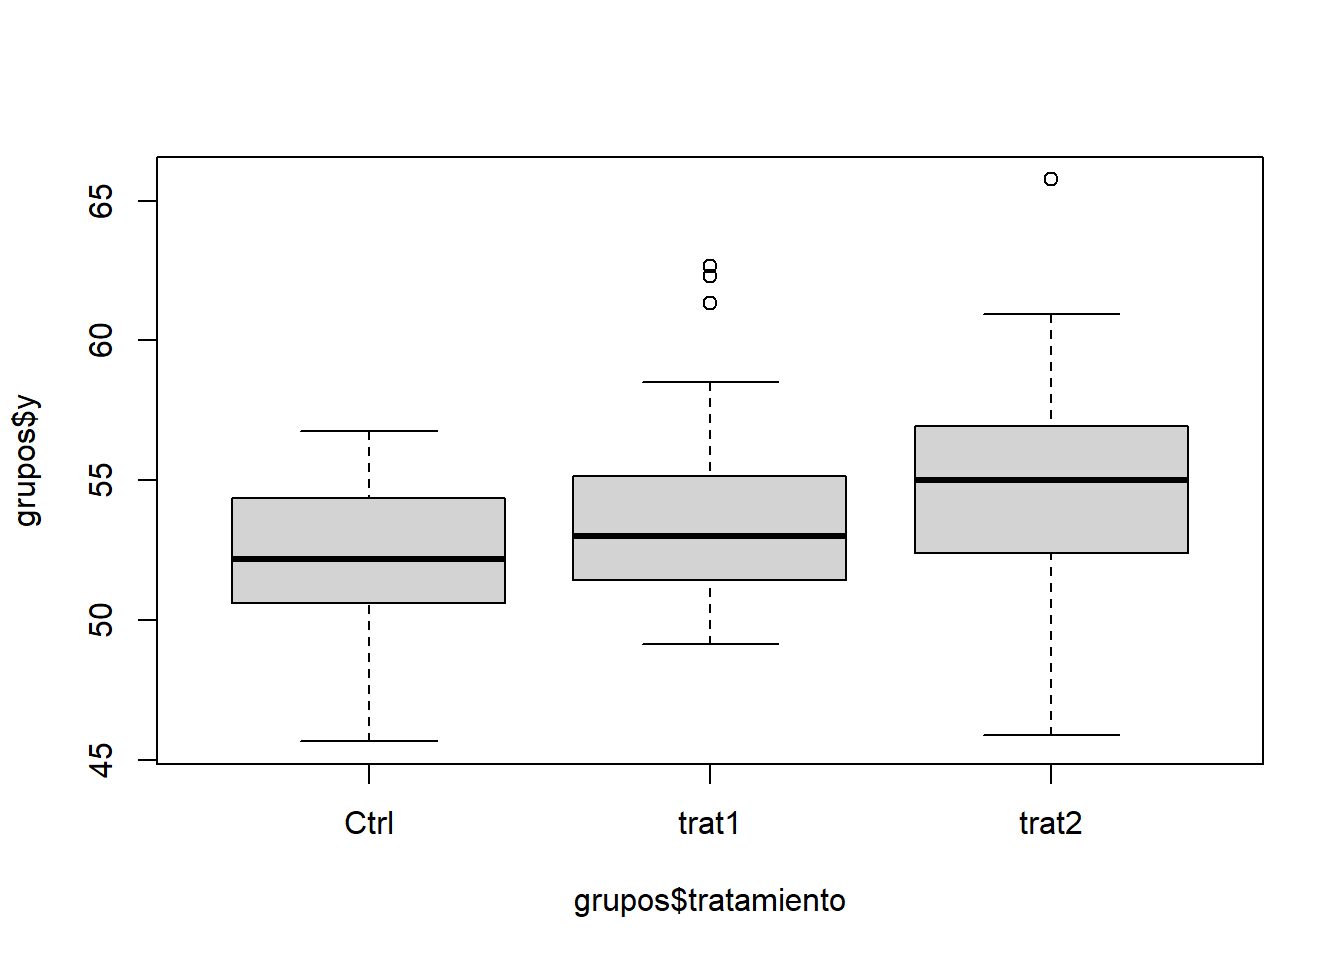
\includegraphics{PractCasa03-full_files/figure-latex/unnamed-chunk-14-1.pdf}

\begin{Shaded}
\begin{Highlighting}[]
\CommentTok{\# Obten los outliers para cada grupo}
\CommentTok{\# con identify\_outliers()}
\NormalTok{outs }\OtherTok{\textless{}{-}}\NormalTok{ grupos }\SpecialCharTok{\%\textgreater{}\%} 
  \FunctionTok{group\_by}\NormalTok{(tratamiento) }\SpecialCharTok{\%\textgreater{}\%} 
  \FunctionTok{identify\_outliers}\NormalTok{(y)}

\CommentTok{\# A2: Elimina los outliers y asigna la tabla limpia con el}
\CommentTok{\# nombre gruposLimpio}
\NormalTok{gruposLimpio }\OtherTok{\textless{}{-}} \FunctionTok{anti\_join}\NormalTok{(grupos, outs)}
\end{Highlighting}
\end{Shaded}

\begin{verbatim}
## Joining, by = c("y", "x1", "x2", "grp", "tratamiento")
\end{verbatim}

\begin{Shaded}
\begin{Highlighting}[]
\CommentTok{\# Verifica si los niveles de tratamiento están balanceados}
\FunctionTok{table}\NormalTok{(gruposLimpio}\SpecialCharTok{$}\NormalTok{tratamiento)}
\end{Highlighting}
\end{Shaded}

\begin{verbatim}
## 
##  Ctrl trat1 trat2 
##    32    29    30
\end{verbatim}

Balancea el estudio:

\begin{Shaded}
\begin{Highlighting}[]
\CommentTok{\# Selecciona de manera aleatoria las observaciones (filas)}
\CommentTok{\# que debes eliminar de gruposLimpio para cada nivel de }
\CommentTok{\# tratamiento y así balancear el ANOVA}
\FunctionTok{set.seed}\NormalTok{(}\DecValTok{12345}\NormalTok{)}
\NormalTok{rCtrl }\OtherTok{\textless{}{-}}\NormalTok{ gruposLimpio }\SpecialCharTok{\%\textgreater{}\%} \FunctionTok{filter}\NormalTok{(tratamiento}\SpecialCharTok{==}\StringTok{"Ctrl"}\NormalTok{) }\SpecialCharTok{\%\textgreater{}\%} \FunctionTok{sample\_n}\NormalTok{(}\DecValTok{3}\NormalTok{)}
\NormalTok{rtrat2 }\OtherTok{\textless{}{-}}\NormalTok{ gruposLimpio }\SpecialCharTok{\%\textgreater{}\%} \FunctionTok{filter}\NormalTok{(tratamiento}\SpecialCharTok{==}\StringTok{"trat2"}\NormalTok{) }\SpecialCharTok{\%\textgreater{}\%} \FunctionTok{sample\_n}\NormalTok{(}\DecValTok{1}\NormalTok{)}

\CommentTok{\# Asigna la base de datos balanceada con el nombre gruposFinal}
\NormalTok{gruposFinal }\OtherTok{\textless{}{-}} \FunctionTok{anti\_join}\NormalTok{(gruposLimpio,rCtrl) }\SpecialCharTok{\%\textgreater{}\%} \FunctionTok{anti\_join}\NormalTok{(.,rtrat2)}
\end{Highlighting}
\end{Shaded}

\begin{verbatim}
## Joining, by = c("y", "x1", "x2", "grp", "tratamiento")
## Joining, by = c("y", "x1", "x2", "grp", "tratamiento")
\end{verbatim}

\begin{Shaded}
\begin{Highlighting}[]
\CommentTok{\# Verifica si realmente está balanceado el ANOVA ahora}
\FunctionTok{table}\NormalTok{(gruposFinal}\SpecialCharTok{$}\NormalTok{tratamiento)}
\end{Highlighting}
\end{Shaded}

\begin{verbatim}
## 
##  Ctrl trat1 trat2 
##    29    29    29
\end{verbatim}

Verifica los supuestos teóricos restantes

\begin{Shaded}
\begin{Highlighting}[]
\CommentTok{\# Realiza el modelamiento lineal}
\NormalTok{mod1 }\OtherTok{\textless{}{-}} \FunctionTok{lm}\NormalTok{(y }\SpecialCharTok{\textasciitilde{}}\NormalTok{ tratamiento, }\AttributeTok{data=}\NormalTok{gruposFinal)}

\CommentTok{\# A3: Verifica la normalidad de los residuales}
\FunctionTok{shapiro.test}\NormalTok{(}\FunctionTok{resid}\NormalTok{(mod1))}
\end{Highlighting}
\end{Shaded}

\begin{verbatim}
## 
##  Shapiro-Wilk normality test
## 
## data:  resid(mod1)
## W = 0.9906, p-value = 0.7915
\end{verbatim}

\begin{Shaded}
\begin{Highlighting}[]
\NormalTok{nortest}\SpecialCharTok{::}\FunctionTok{ad.test}\NormalTok{(}\FunctionTok{resid}\NormalTok{(mod1))}
\end{Highlighting}
\end{Shaded}

\begin{verbatim}
## 
##  Anderson-Darling normality test
## 
## data:  resid(mod1)
## A = 0.19844, p-value = 0.8838
\end{verbatim}

\begin{Shaded}
\begin{Highlighting}[]
\CommentTok{\# A4: Verifica la homogeneidad de varianzas}
\FunctionTok{bartlett.test}\NormalTok{(y }\SpecialCharTok{\textasciitilde{}}\NormalTok{ tratamiento, }\AttributeTok{data=}\NormalTok{gruposFinal)}
\end{Highlighting}
\end{Shaded}

\begin{verbatim}
## 
##  Bartlett test of homogeneity of variances
## 
## data:  y by tratamiento
## Bartlett's K-squared = 2.2933, df = 2, p-value = 0.3177
\end{verbatim}

Realiza el ANOVA final y su respectivo post hoc si es necesario

\begin{Shaded}
\begin{Highlighting}[]
\CommentTok{\# Modelo final }
\FunctionTok{anova}\NormalTok{(mod1)}
\end{Highlighting}
\end{Shaded}

\begin{verbatim}
## Analysis of Variance Table
## 
## Response: y
##             Df Sum Sq Mean Sq F value    Pr(>F)    
## tratamiento  2 111.94  55.968  7.7188 0.0008368 ***
## Residuals   84 609.07   7.251                      
## ---
## Signif. codes:  0 '***' 0.001 '**' 0.01 '*' 0.05 '.' 0.1 ' ' 1
\end{verbatim}

\begin{Shaded}
\begin{Highlighting}[]
\CommentTok{\# Post Hoc}
\FunctionTok{TukeyHSD}\NormalTok{(}\FunctionTok{aov}\NormalTok{(mod1))}
\end{Highlighting}
\end{Shaded}

\begin{verbatim}
##   Tukey multiple comparisons of means
##     95% family-wise confidence level
## 
## Fit: aov(formula = mod1)
## 
## $tratamiento
##                 diff        lwr      upr     p adj
## trat1-Ctrl  1.258966 -0.4282642 2.946195 0.1824074
## trat2-Ctrl  2.774483  1.0872530 4.461712 0.0005173
## trat2-trat1 1.515517 -0.1717125 3.202747 0.0873564
\end{verbatim}

\textbf{P1:} \emph{¿Existen diferencias significativas entre los
grupos?}

\textbf{Rpta/.} el Pr(\textgreater F) de la variable tratamiento en el
resultado del ANOVA es significativo: 0.0008368 ***

\textbf{P2:} \emph{¿Cuál es el tratamiento que generó un mayor
incremento del promedio de la variable y?}

\textbf{Rpta/.} Al ver el resultado del post hoc, lo primero que se debe
revisar es la significancia de las diferencias entre los tratamientos.
Las diferencias entre niveles que no son significativos nos indican que
no hay evidencia estadística que soporte que dichas restas son
diferentes de cero. Por lo que no se puede decir que hay diferencias
estadísticas entre los niveles en cuestión. Eso sucede con las restas
entre los promedios de \texttt{trat1-Ctrl} y \texttt{trat2-trat1}. Por
lo que la única resta de promedios significativa fue
\texttt{trat2-Ctrl}= 2.77 (p-valor 0.0005). Interpretando, decimos que:
\texttt{trat2} genera un promedio mayor a \texttt{Ctrl}, debido a que la
resta de ambos es positiva. Por el contrario, no hay evidencia de que
existan diferencias entre \texttt{trat1-Ctrl} y \texttt{trat2-trat1}. En
consecuencia, \texttt{trat2} es el tratamiento que genera un mayor
incremento de \texttt{y}.

\hypertarget{ejercicio-7-poder-de-anuxe1lisis}{%
\section{\texorpdfstring{\textbf{Ejercicio 7: Poder de
análisis}}{Ejercicio 7: Poder de análisis}}\label{ejercicio-7-poder-de-anuxe1lisis}}

Conocer el poder de un análisis nos puede ayudar a decidir si podemos
incrementar el n muestral para obtener un resultado mucho más fiable,
estadísticamente hablando.

Desarrolla lo siguiente:

\begin{Shaded}
\begin{Highlighting}[]
\CommentTok{\# Calcula el tamaño del efecto del ANOVA balanceado}
\CommentTok{\# qaue desarrollaste anteriormente (redondea el valor a dos decimales)}
\NormalTok{rstatix}\SpecialCharTok{::}\FunctionTok{eta\_squared}\NormalTok{(}\FunctionTok{anova}\NormalTok{(mod1)) }\SpecialCharTok{\%\textgreater{}\%} \FunctionTok{round}\NormalTok{(}\DecValTok{2}\NormalTok{)}
\end{Highlighting}
\end{Shaded}

\begin{verbatim}
## tratamiento 
##        0.16
\end{verbatim}

\begin{Shaded}
\begin{Highlighting}[]
\CommentTok{\# Calcula el poder del análisis de dicho ANOVA}
\FunctionTok{pwr.anova.test}\NormalTok{(}\AttributeTok{k=}\DecValTok{3}\NormalTok{, }\AttributeTok{sig.level =} \FloatTok{0.05}\NormalTok{, }\AttributeTok{f =} \FloatTok{0.13}\NormalTok{, }\AttributeTok{n=}\DecValTok{29}\NormalTok{)}
\end{Highlighting}
\end{Shaded}

\begin{verbatim}
## 
##      Balanced one-way analysis of variance power calculation 
## 
##               k = 3
##               n = 29
##               f = 0.13
##       sig.level = 0.05
##           power = 0.1708106
## 
## NOTE: n is number in each group
\end{verbatim}

\begin{Shaded}
\begin{Highlighting}[]
\CommentTok{\# Identifica cuál sería el n muestral necesario para obtener}
\CommentTok{\# un poder de análisis de 80\%}
\FunctionTok{pwr.anova.test}\NormalTok{(}\AttributeTok{k=}\DecValTok{3}\NormalTok{, }\AttributeTok{sig.level =} \FloatTok{0.05}\NormalTok{, }\AttributeTok{f =} \FloatTok{0.16}\NormalTok{, }\AttributeTok{power =} \FloatTok{0.8}\NormalTok{)}
\end{Highlighting}
\end{Shaded}

\begin{verbatim}
## 
##      Balanced one-way analysis of variance power calculation 
## 
##               k = 3
##               n = 126.4556
##               f = 0.16
##       sig.level = 0.05
##           power = 0.8
## 
## NOTE: n is number in each group
\end{verbatim}

\hypertarget{ejercicio-8-anova-no-balanceado-una-vuxeda}{%
\section{\texorpdfstring{\textbf{Ejercicio 8: ANOVA No Balanceado (una
vía)}}{Ejercicio 8: ANOVA No Balanceado (una vía)}}\label{ejercicio-8-anova-no-balanceado-una-vuxeda}}

Trabajemos el ANOVA no balanceado del \textbf{Ejercicio 6} y veamos qué
diferencias encontramos con los resultados del ANOVA balanceado. Como
aquí no necesitamos utilizar los niveles de \texttt{tratamiento} con el
mismo n muestral, usaremos la variable creada en el ambiente de R
llamada \texttt{gruposLimpio}.

\begin{Shaded}
\begin{Highlighting}[]
\CommentTok{\# Realiza el modelamiento lineal}
\NormalTok{mod2 }\OtherTok{\textless{}{-}} \FunctionTok{lm}\NormalTok{(y }\SpecialCharTok{\textasciitilde{}}\NormalTok{ tratamiento, }\AttributeTok{data=}\NormalTok{gruposLimpio)}

\CommentTok{\# A3: Verifica la normalidad de los residuales}
\FunctionTok{shapiro.test}\NormalTok{(}\FunctionTok{resid}\NormalTok{(mod2))}
\end{Highlighting}
\end{Shaded}

\begin{verbatim}
## 
##  Shapiro-Wilk normality test
## 
## data:  resid(mod2)
## W = 0.99076, p-value = 0.7795
\end{verbatim}

\begin{Shaded}
\begin{Highlighting}[]
\NormalTok{nortest}\SpecialCharTok{::}\FunctionTok{ad.test}\NormalTok{(}\FunctionTok{resid}\NormalTok{(mod2))}
\end{Highlighting}
\end{Shaded}

\begin{verbatim}
## 
##  Anderson-Darling normality test
## 
## data:  resid(mod2)
## A = 0.20766, p-value = 0.8625
\end{verbatim}

\begin{Shaded}
\begin{Highlighting}[]
\CommentTok{\# A4: Verifica la homogeneidad de varianzas}
\FunctionTok{bartlett.test}\NormalTok{(y }\SpecialCharTok{\textasciitilde{}}\NormalTok{ tratamiento, }\AttributeTok{data=}\NormalTok{gruposLimpio)}
\end{Highlighting}
\end{Shaded}

\begin{verbatim}
## 
##  Bartlett test of homogeneity of variances
## 
## data:  y by tratamiento
## Bartlett's K-squared = 2.1026, df = 2, p-value = 0.3495
\end{verbatim}

\begin{Shaded}
\begin{Highlighting}[]
\CommentTok{\# Modelo final }
\FunctionTok{anova}\NormalTok{(mod2)}
\end{Highlighting}
\end{Shaded}

\begin{verbatim}
## Analysis of Variance Table
## 
## Response: y
##             Df Sum Sq Mean Sq F value   Pr(>F)   
## tratamiento  2 105.97  52.985   7.237 0.001231 **
## Residuals   88 644.28   7.321                    
## ---
## Signif. codes:  0 '***' 0.001 '**' 0.01 '*' 0.05 '.' 0.1 ' ' 1
\end{verbatim}

\begin{Shaded}
\begin{Highlighting}[]
\CommentTok{\# Post Hoc}
\FunctionTok{TukeyHSD}\NormalTok{(}\FunctionTok{aov}\NormalTok{(mod2))}
\end{Highlighting}
\end{Shaded}

\begin{verbatim}
##   Tukey multiple comparisons of means
##     95% family-wise confidence level
## 
## Fit: aov(formula = mod2)
## 
## $tratamiento
##                 diff         lwr      upr     p adj
## trat1-Ctrl  1.006185 -0.64766568 2.660036 0.3198435
## trat2-Ctrl  2.600542  0.96121431 4.239869 0.0008204
## trat2-trat1 1.594356 -0.08549883 3.274211 0.0665400
\end{verbatim}

En estos casos de anovas de una vía, balanceados o no, el algoritmo de
la función \texttt{anova()} es lo suficientemente robusto para mantener
los resultados entre ambos. Esto no es igual para ANOVAs de dos vías.

\end{document}
